\documentclass[conference]{IEEEtran}
\IEEEoverridecommandlockouts
%Template version as of 6/27/2024

\usepackage{cmap}
\usepackage[T1]{fontenc}
\usepackage{cite}
\usepackage{amsmath,amssymb,amsfonts}
\usepackage{algorithmic}
\usepackage{graphicx}
\usepackage{textcomp}
\usepackage{xcolor}
\usepackage{subcaption}
\usepackage{booktabs}
\usepackage{url}
\usepackage{microtype}
\usepackage{listings}
\usepackage{float}
\usepackage{multirow}

\def\BibTeX{{\rm B\kern-.05em{\sc i\kern-.025em b}\kern-.08em
		T\kern-.1667em\lower.7ex\hbox{E}\kern-.125emX}}

\lstset{
	basicstyle=\ttfamily\footnotesize,
	breaklines=true,
	breakatwhitespace=true,
	frame=single,
	columns=fullflexible,
	keepspaces=true
}

\begin{document}

\title{The Cloud EC2 Sweet Spot: Cost Optimization and Scaling Strategies for Video-as-a-Service Workloads}

\author{
	\IEEEauthorblockN{Anonymous Authors}
	\IEEEauthorblockA{\textit{Anonymous Affiliation} \\
		Anonymous City, Anonymous Country \\
		anonymous@example.com}
}

\maketitle

% -----------------------------------------------------------------------
% ABSTRACT
% -----------------------------------------------------------------------
% Notes on numbers used here:
%   - 57.3%--93.3%: T-family Phase 3.1 range (serial=57.3%, parallel=93.3%)
%     used as the unoptimized baseline family.
%   - 89.4% cost reduction: cross-family comparison,
%     t3.micro cluster ($0.00211) vs m5.4xlarge vertical ($0.01997)
%     = (0.01997-0.00211)/0.01997
%   - 87.5% cost reduction: cross-family comparison,
%     t3.micro cluster ($0.00211) vs c5.4xlarge vertical ($0.01689)
%     = (0.01689-0.00211)/0.01689
%   - 1.28x speedup (cross-family): 10x t3.micro cluster (1.22 min)
%     vs m5.4xlarge vertical (1.56 min) = 1.56/1.22
%     NOTE: 10x m5.large cluster also achieves 1.22 min (same speedup,
%     intra-family). Both comparisons yield 1.28x, but the abstract
%     attributes this to the t3.micro cross-family comparison.
%   - 1.26x speedup over c5.4xlarge: 10x c5.large cluster (1.18 min)
%     vs c5.4xlarge vertical (1.49 min) = 1.49/1.18
\begin{abstract}
Picking the right EC2 instance for video transcoding turns out to be harder than AWS pricing pages make it look. A burstable \texttt{t3.micro} can be 29$\times$ cheaper per encoding job than a Compute-Optimized node---but scaling out na\"{i}vely wipes that gain: when every worker must install its own software stack, provisioning eats up to 93.3\% of wall-clock time and parallelism buys nothing.

We ran over 5\,700 controlled experiments across 15 instance types (Burstable, General Purpose, Compute-Optimized, and ARM Graviton), three codecs (H.264, H.265, VP9), and three scaling strategies, repeating each configuration 30 times. The bottleneck was always the same: getting the instance ready, not running the encoder. Pre-baking dependencies into a custom AMI removed that overhead and let a 10-node \texttt{t3.micro} cluster beat a single \texttt{m5.4xlarge} by $1.28\times$ at 89.4\% lower compute cost (62\% after accounting for burst-credit surcharges). The same pattern appeared within non-burstable families (10$\times$ \texttt{m5.large} vs.\ \texttt{m5.4xlarge}), ruling out credit mechanics as the explanation. A chunk-size sweep at three resolutions showed that the optimal partition length shifts from 60\,s at 240p to 30\,s at 720p and 1080p, where encoding time outweighs provisioning. Once compute was optimized, data-egress charges emerged as the dominant remaining cost. ARM Graviton clusters matched x86 H.265 throughput at lower per-hour rates. Together, these results give practitioners concrete, statistically grounded rules for sizing and scheduling cloud transcoding clusters.
\end{abstract}

\begin{IEEEkeywords}
Cloud Computing; Video-as-a-Service; Cost Optimization; Video Transcoding; Horizontal Scaling; Provisioning Overhead; Elasticity; ARM Graviton
\end{IEEEkeywords}

% -----------------------------------------------------------------------
% INTRODUCTION
% -----------------------------------------------------------------------
\section{Introduction}

Video transcoding is one of the most CPU-hungry tasks in media delivery, and cloud platforms are where most of it runs today. For Video-as-a-Service (VaaS) operators---whether they serve streaming, surveillance, or large-scale content distribution---which EC2 instance family they pick has a direct impact on margins~\cite{b1,b17}.

The usual advice is to reach for Compute-Optimized instances when encoding is the bottleneck, on the assumption that faster hardware means lower cost per job. In practice, things are less straightforward: under the burst conditions and codecs we tested, Burstable instances turned out to be up to 29$\times$ more cost-efficient despite being slower in absolute terms. The catch is that this advantage evaporates at scale---not because of a hardware ceiling, but because of a systems-level problem: provisioning overhead, the ``cold start'' delay before any encoding even begins.

Previous studies have tackled cloud benchmarking~\cite{b1}, HPC workloads on cloud infrastructure~\cite{b3}, and multi-cloud scheduling~\cite{b20}, yet cost optimization across different instance families for media workloads remains underexplored. Comparing Burstable, General Purpose, and Compute-Optimized tiers is tricky in its own right: burstable instances bring CPU credit mechanics and different pricing floors that existing benchmarks have not measured under realistic video encoding loads. We focus on H.264, H.265, and VP9---the three codecs that still dominate commercial pipelines. Newer standards like VVC promise better compression, but limited hardware acceleration and unresolved licensing on current EC2 generations keep them outside the scope of most production deployments.

We test AWS T, M, and C instance families, covering both x86 and ARM Graviton architectures, under three scaling strategies (serial, horizontal, vertical). Four questions drive the work:
\begin{enumerate}
\item[\textbf{RQ1.}] How do cost-performance profiles differ across instance families, CPU architectures, and codecs (H.264, H.265, VP9)?
\item[\textbf{RQ2.}] How does provisioning overhead constrain parallel encoding efficiency, and what fraction of total execution time does it represent?
\item[\textbf{RQ3.}] Can provisioning optimizations---specifically pre-built AMIs---make small-instance clusters competitive with or superior to vertical scaling, in both time and cost?
\item[\textbf{RQ4.}] How do regional pricing disparities and network egress costs define the economic floor of optimized VaaS deployments?
\end{enumerate}

The short answer: provisioning latency---not compute capacity---is what limits horizontal scaling of short-lived transcoding jobs. In unoptimized deployments, it ate 57.3\%--93.3\% of total wall-clock time across T-family configurations. Building a workload-optimized AMI removes most of that overhead, and the economics flip: a 10-node \texttt{t3.micro} cluster beats a single \texttt{m5.4xlarge} by $1.28\times$ at 89.4\% lower compute cost (62\% after accounting for CPU credit surcharges). The same $1.28\times$ speedup shows up intra-family (10$\times$ \texttt{m5.large} vs.\ \texttt{m5.4xlarge}), which rules out cross-family comparison artifacts. A chunk size sweep and an egress cost model round out the picture: once compute is optimized, data transfer takes over as the dominant cost.

% -----------------------------------------------------------------------
% RELATED WORKS
% -----------------------------------------------------------------------
\section{Related Works}
\label{rel_works}

Work on cloud resource optimization for media workloads falls roughly into two camps: general cloud benchmarking and provisioning on one side, and video-encoding-specific studies on the other. Neither camp has looked at what we address here---the interaction between instance family selection and provisioning strategy for repetitive, divisible encoding jobs. Infrastructure studies tend to treat workloads as monolithic tasks; encoding studies optimize throughput-per-dollar. But for short-lived, horizontally-scaled video chunks, provisioning latency is a hidden constant that both communities have largely ignored across cloud instance families.

On the infrastructure side, researchers have benchmarked cloud instances across workload classes~\cite{b1}, compared cloud and supercomputer execution for HPC~\cite{b3}, and built cost-driven provisioning for scientific computing~\cite{b2}. Resource management surveys~\cite{b4} and thread scalability studies~\cite{b23} add useful context. Still, none of these papers measure the environment provisioning overhead that hurts horizontally scaled, chunk-based VaaS deployments.

On the encoding side, Moina-Rivera et al.~\cite{b22} survey cloud and edge transcoding architectures, and Katsenou et al.~\cite{b8} look at energy-codec trade-offs on embedded devices. Jiang et al.~\cite{b20} propose a multi-cloud cost-aware scheduler for big-data pipelines but say little about video-specific workload properties. The closest predecessor to our parallelism approach is ExCamera~\cite{excamera} (Fouladi et al.), which reached 60--300$\times$ speedups through fine-grained serverless (AWS Lambda) parallelism. We borrow the chunked-parallelism idea but ask a different question---what does ephemeral compute actually cost on EC2, where VM and environment provisioning creates bottlenecks that do not exist in serverless, and where na\"{i}ve parallelism can actually \emph{degrade} performance, turning the ``more parallelism is always better'' assumption on its head. AWS Elemental MediaConvert~\cite{awsmediaconvert} sidesteps provisioning overhead entirely as a managed service, but its black-box pricing tiers remove any instance-level control over margins.

Spot instance pricing~\cite{b21,b19} can cut costs beyond what we report, but preemption risk makes it hard to guarantee the deterministic latency that VaaS SLAs require, so we leave that comparison for future work. Cloud performance variability is well-documented~\cite{b18,b10}---which is why we ran 30 trials per configuration. Our chunked workload decomposition builds on ideas from the fog-cloud~\cite{b12} and distributed scheduling~\cite{b13} literature.

Table~\ref{tab:comparative_analysis} summarizes the positioning of our work relative to related research.

\begin{table*}[!htbp]
	\centering
	\caption{Comparison of related works in cloud resource optimization and video processing}
	\label{tab:comparative_analysis}
	\begin{tabular}{|p{0.15\linewidth}|p{0.18\linewidth}|p{0.26\linewidth}|p{0.30\linewidth}|}
		\hline
		\textbf{Study} & \textbf{Focus} & \textbf{Contributions} & \textbf{Limitations for VaaS} \\
		\hline
		Álvarez et al. \cite{b2} & Scientific workloads & Cost-aware provisioning for compute-intensive services & Lacks media-specific transient workload analysis \\
		\hline
		Dancheva et al. \cite{b3} & HPC cloud benchmarking & Cloud vs.\ supercomputer execution (CFD on EC2) & HPC-centric; ignores video encoding economics and chunking \\
		\hline
		Jiang et al. \cite{b20} & Multi-cloud scheduling & Cost-aware framework for cross-cloud workflows & Big-data focus; does not address granular VaaS chunking constraints \\
		\hline
		Maas et al. \cite{b1,b23} & Broad cloud benchmarking & Instance performance and thread scalability analysis & Generic workloads; misses provisioning penalties for short-lived tasks \\
		\hline
		Katsenou et al. \cite{b8} & Energy efficiency & Codec energy analysis on embedded devices & Embedded focus; not applicable to IaaS cloud economics \\
		\hline
		Moina-Rivera et al. \cite{b22} & Cloud/Edge video & Literature review of media encoding architectures & Theoretical survey; no empirical multi-family IaaS benchmarking \\
		\hline
		Zabrovskiy et al. \cite{b21} & Spot instance costs & FSpot scheduling heuristic for minimal cost encoding & Volatile spot instances introduce preemption risk \\
		\hline
		Fouladi et al. \cite{excamera} & Serverless video & Chunk-parallel encoding via Lambda (ExCamera) & Serverless model; abstracts away VM provisioning and IaaS economics \\
		\hline
		Our Work & IaaS video transcoding & Cost-performance of chunked encoding across T, M, C families (x86 and ARM); AMI mitigation; holistic egress cost modeling & Quantifies provisioning overhead; proves AMI mitigation; provides actionable VaaS instance-selection guidelines \\
		\hline
	\end{tabular}
\end{table*}

% -----------------------------------------------------------------------
% EXPERIMENTAL METHODOLOGY
% -----------------------------------------------------------------------
\section{Experimental Methodology}
\label{met}

The study has four phases, each feeding into the next. Phase~1 characterizes the hardware environment; Phase~2 benchmarks raw encoding performance across the instance space; Phase~3 tests scaling strategies under realistic pipeline conditions; Phase~4 quantifies how chunk duration and egress costs affect the bottom line. All experiments ran on AWS in \texttt{us-east-1} (N. Virginia); we replicated selected configurations in \texttt{sa-east-1} (São Paulo) to check for regional price effects.

\subsection{Phase 1: Validation of Processor Homogeneity}

AWS does not guarantee that every instance of a given type runs on the same processor model. To measure this variability before running benchmarks, we launched 100 instances of each configuration (T, M, C families) across all six availability zones (a--f) in \texttt{us-east-1}, each running Ubuntu 22.04 LTS, and read \texttt{/proc/cpuinfo} on every one.

The results confirmed real heterogeneity, in line with prior cloud studies~\cite{b2, b5, b6, b7}: \texttt{t3.micro} in zone~\texttt{a} was 98\% Xeon~8259CL / 2\% Xeon~8175M; \texttt{m5.large} in zone~\texttt{c} split 60\%/40\% between 8259CL and 8175M; \texttt{c5.large} in zone~\texttt{b} split 74\%/26\% between 8275CL and 8124M. ARM Graviton instances (\texttt{t4g}, \texttt{m7g}, \texttt{c7g}) were fully homogeneous (100\%).

To keep CPU model from confounding Phase~3 results, our provisioning scripts check \texttt{/proc/cpuinfo} as soon as SSH is up. If the instance landed on the wrong processor, it gets terminated and relaunched; the loop continues until the target model is confirmed. For T-family (98\% dominant), this almost always works on the first try; M and C families (60--74\% dominant) needed extra retries in a minority of cases. All 30 runs per configuration ended up on the same CPU model. Phase~3 ARM experiments use Graviton~3 only (\texttt{m7g.large}, \texttt{c7g.large}); we validated \texttt{t4g} (Graviton~2) but excluded it from scaling tests because its credit mechanics would confound the comparison.

\subsection{Phase 2: Initial Performance Benchmarks}

Phase~2 measures raw encoding performance across all 15 instance types with a containerized FFmpeg environment (H.264/AVC, H.265/HEVC, VP9).

The workload is a 320$\times$240 (240p) test sequence with mixed motion. We chose this resolution deliberately: it keeps the bottleneck in the CPU and codec thread scheduler rather than in I/O or memory bandwidth, isolating instance-level compute differences that would get masked at 1080p or 4K by memory and disk pressure on smaller instances. Segments are 30 seconds---long enough that process initialization (container startup, FFmpeg loading) is negligible relative to encoding time, short enough to allow 30 replications per configuration without the experiment taking forever. Each condition ran 30 times. Encoding used:

\begin{center}
	{\ttfamily\scriptsize
		\fbox{
			\begin{minipage}{0.9\linewidth}
				ffmpeg -i input.mp4 -c:v <codec> -preset slow -b:v 2M \\
				\hspace{15pt}-threads <n> output.mp4
			\end{minipage}
		}
	}
\end{center}

The \texttt{<codec>} parameter evaluated \texttt{libx264}, \texttt{libx265},
and \texttt{libvpx-vp9}. The \texttt{<n>} parameter was tested with 1, 3, 5, and 10 threads for all instances, and additionally with 16 threads for \texttt{m5.4xlarge} and \texttt{c5.4xlarge} (the only configurations with 16 vCPUs). Encoding duration was recorded and cost calculated based on
instance pricing.

\subsection{Phase 3: Horizontal vs. Vertical Scaling Analysis}

Phase~3 takes the instance ranking from Phase~2 and asks a practical pipeline question: for a 10-minute video, is it better to scale horizontally (ten parallel small instances) or vertically (one large instance)? Ten minutes is long enough to need chunked parallel processing but short enough to run repeated end-to-end trials.

We compare three configurations across all T, M, and C families (x86 and ARM): horizontal (10$\times$ small instance), vertical (single large instance), and serial (1$\times$ small instance, full video). We also replicated selected configurations in \texttt{sa-east-1} to check regional pricing effects.

The scaling investigation has two sub-phases. Phase~3.1 (Dynamic Provisioning) uses stock Ubuntu images with post-boot FFmpeg installation---the unoptimized baseline. Phase~3.2 (Optimized Provisioning) uses a pre-configured custom AMI with FFmpeg already installed, measuring the best case once runtime setup costs are gone. Both phases record end-to-end wall-clock time and total cost.

\subsection{Phase 3 Extended Evaluation: ARM Graviton and Regional Pricing}

We extended Phase~3 in two directions to test how well the findings generalize. First, two ARM Graviton 3 instances (\texttt{m7g.large} and \texttt{c7g.large}) were run alongside their x86 counterparts using the same horizontal and serial strategies. The ARM experiments also added H.265 (libx265) and VP9 (libvpx-vp9) to see how codec-specific performance differs across architectures. We applied the same $n=30$ repetition protocol and terminate-and-retry CPU verification from Phase~1.

Second, we replicated the horizontal scaling evaluation in \texttt{sa-east-1} (S\~{a}o Paulo) for three representative instances (\texttt{t3.micro}, \texttt{m5.large}, \texttt{c5.large}) using H.264, to see how regional pricing changes the cost-performance picture from the primary \texttt{us-east-1} experiments.

\subsection{Phase 4: Chunk Size Sensitivity and Cost Analysis}

Phase~4 adds two analyses on top of the scaling results. First, a chunk size sensitivity analysis looks at how segment duration $c$ affects total wall-clock time $T(c)$ for a video of length $L$ encoded across $N = \lceil L/c \rceil$ parallel instances. Pipeline time breaks down into four observable parts: segmentation ($t_{\text{seg}}$), provisioning and boot latency of the slowest node ($\max_i t_{\text{prov},i}$), per-chunk encoding ($t_{\text{enc}}(c)$), and output merge ($t_{\text{merge}}$). We tested three chunk durations: 30\,s ($N=20$), 60\,s ($N=10$), and 120\,s ($N=5$). Second, a network cost model captures the economic impact of data egress. Total pipeline cost $C_{\text{total}}$ splits into compute provisioning cost $C_{\text{comp}} = \sum_{i=1}^{N} R_{\text{inst}} \times T_i$ and outbound transfer cost $C_{\text{net}} = R_{\text{egress}} \times D_{\text{out}}$, formalized in Eq.~\ref{eq:cost_model} and validated against empirical measurements in Section~\ref{results-phase4}.

All execution times were recorded at millisecond resolution. Each configuration was repeated $n=30$ times in both Phase~2 and Phase~3. With $n=30$, the Central Limit Theorem gives us a near-normal sampling distribution of the mean, so Welch's t-test is appropriate even when the raw data are not perfectly normal. We report descriptive statistics and 95\% Confidence Intervals (Student's t-distribution) for every configuration. Statistical tests include Shapiro-Wilk for normality, Levene's for variance homogeneity, and Welch's t-tests for group comparisons.

% -----------------------------------------------------------------------
% EXPERIMENTAL RESULTS
% -----------------------------------------------------------------------
\section{Experimental Results and Analysis}
\label{experiments}

Results follow the four-phase structure laid out in Section~\ref{met}.

\subsection{Phase 1 Results: Processor Homogeneity Validation}

As expected from prior cloud benchmarking work~\cite{b5, b6}, AWS does not deliver the same processor model every time you request an instance type. T-family (\texttt{t3.micro}) in zone~\texttt{a} was 98\% Intel Xeon Platinum 8259CL / 2\% 8175M---effectively homogeneous. M and C families, though, showed a 60\%/40\% split between processor models, which is enough to confound latency comparisons if left uncontrolled.

For Phase~3, we pinned execution to the dominant processor per family: 8259CL for M-type, 8275CL for C-type. Any instance that launched on the wrong processor was terminated and relaunched; the loop ran until \texttt{/proc/cpuinfo} confirmed the target model. Every one of the 30 runs per configuration ended up on the same CPU model.

\subsection{Phase 2 Results: Initial Performance Benchmarks}

Phase~2 benchmarks H.264, H.265, and VP9 across all 15 instance types at multiple thread counts, giving us the baseline cost-performance map that drives Phase~3 scaling decisions. Each configuration ran 30 times on isolated 30-second segments; we report Compression Time (seconds), Efficiency (Eq.~\ref{eq:efficiency}), and Total Cost (Eq.~\ref{eq:total_cost}).

\subsubsection{Efficiency and Cost Calculation}

These two metrics are inverses of each other: $\text{Efficiency} = 1/\text{Total Cost}$, where $\text{cost}_{(h)}$ comes from Table~\ref{tab:experimental_configurations} and $\text{time}_{(s)}$ is the measured encoding duration. Total Cost gives a dollar figure per operation; Efficiency gives a relative index that is easier to read when values span orders of magnitude.

\begin{equation}
	\text{Efficiency} = \frac{1}{(\text{cost}_{(h)}/3600) \times \text{time}_{(s)}}
	\label{eq:efficiency}
\end{equation}

\begin{equation}
	\text{Total Cost} = (\text{cost}_{(h)}/3600) \times \text{time}_{(s)}
	\label{eq:total_cost}
\end{equation}

\begin{table}[!htbp]
	\centering
	\caption{Experimental instance configurations and on-demand pricing (Linux, shared tenancy). All prices retrieved March 2026 via AWS Pricing API.}
	\label{tab:experimental_configurations}
	\begin{tabular}{|l|c|c|c|c|}
		\hline
		\textbf{Instance} & \textbf{vCPU} & \textbf{RAM(gb)} & \textbf{\$/hr us-east-1} & \textbf{\$/hr sa-east-1} \\
		\hline
		\multicolumn{5}{|l|}{\textit{Burstable (T-family)}} \\
		\hline
		\texttt{t2.micro}   & 1  & 1  & 0.0116 & 0.0186 \\
		\texttt{t3.micro}   & 2  & 1  & 0.0104 & 0.0168 \\
		\texttt{t3.small}   & 2  & 2  & 0.0208 & 0.0336 \\
		\texttt{t3.medium}  & 2  & 4  & 0.0416 & 0.0672 \\
		\texttt{t3.large}   & 2  & 8  & 0.0832 & 0.1344 \\
		\texttt{t3.xlarge}  & 4  & 16 & 0.1664 & 0.2688 \\
		\texttt{t3.2xlarge} & 8  & 32 & 0.3328 & 0.5376 \\
		\hline
		\multicolumn{5}{|l|}{\textit{General Purpose (M5-family, x86)}} \\
		\hline
		\texttt{m5.large}   & 2  & 8  & 0.0960 & 0.1530 \\
		\texttt{m5.xlarge}  & 4  & 16 & 0.1920 & 0.3060 \\
		\texttt{m5.2xlarge} & 8  & 32 & 0.3840 & 0.6120 \\
		\texttt{m5.4xlarge} & 16 & 64 & 0.7680 & 1.2240 \\
		\hline
		\multicolumn{5}{|l|}{\textit{Compute Optimized (C5-family, x86)}} \\
		\hline
		\texttt{c5.large}   & 2  & 4  & 0.0850 & 0.1310 \\
		\texttt{c5.xlarge}  & 4  & 8  & 0.1700 & 0.2620 \\
		\texttt{c5.2xlarge} & 8  & 16 & 0.3400 & 0.5240 \\
		\texttt{c5.4xlarge} & 16 & 32 & 0.6800 & 1.0480 \\
		\hline
		\multicolumn{5}{|l|}{\textit{ARM Graviton3 (M7g/C7g-family, aarch64)}} \\
		\hline
		\texttt{m7g.large}  & 2  & 8  & 0.0816 & 0.1301 \\
		\texttt{c7g.large}  & 2  & 4  & 0.0725 & 0.1111 \\
		\hline
	\end{tabular}
\end{table}

\subsubsection{Performance Analysis}

Table~\ref{tab:final_comparison_consistent} presents descriptive statistics for
Compression Time, Efficiency, and Total Cost across all experimental
configurations.

\begin{table*}[h]
	\centering
	\caption{Descriptive statistics for compression time (seconds), efficiency, and total cost across all experimental configurations}
	\label{tab:final_comparison_consistent}
	\resizebox{\textwidth}{!}{
		\begin{tabular}{ll|rrrrr|rrrrr|rrrrr}
			\toprule
			& & \multicolumn{5}{c|}{H.264} & \multicolumn{5}{c|}{H.265 (libx265)} & \multicolumn{5}{c}{VP9 (libvpx-vp9)} \\
			\cmidrule(lr){3-7} \cmidrule(lr){8-12} \cmidrule(lr){13-17}
			& & \multicolumn{4}{c}{Compression Time (s)} & \multicolumn{1}{c|}{Eff. | Cost (\$)} & \multicolumn{4}{c}{Time (s)} & \multicolumn{1}{c|}{Eff. | Cost (\$)} & \multicolumn{4}{c}{Time (s)} & \multicolumn{1}{c}{Eff. | Cost (\$)} \\
			Instance Type & Threads & Median & Std & Min & Max & (Median) & Median & Std & Min & Max & (Median) & Median & Std & Min & Max & (Median) \\
			\midrule
			t2.micro & 1 thread & \textbf{2.6379} & 0.0125 & 2.6125 & 2.6625 & \textbf{117,647} | \textbf{0.0000085} & 5.0732 & 0.0259 & 5.0227 & 5.1136 & 61,173 | 0.0000163 & 15.1053 & 0.0559 & 15.0461 & 15.2922 & 20,545 | 0.0000487 \\
			t2.micro & 3 thread & 2.7737 & 0.0211 & 2.7433 & 2.8485 & 111,889 | 0.0000089 & 5.0143 & 0.0293 & 4.9592 & 5.1073 & 61,892 | 0.0000162 & \textbf{14.7549} & 0.0470 & 14.7042 & 14.9585 & \textbf{21,033} | \textbf{0.0000475} \\
			t2.micro & 5 thread & 2.7059 & 0.0109 & 2.6892 & 2.7321 & 114,693 | 0.0000087 & 4.8827 & 0.0239 & 4.8423 & 4.9416 & 63,560 | 0.0000157 & 15.4129 & 0.0900 & 15.3474 & 15.7989 & 20,135 | 0.0000497 \\
			t2.micro & 10 thread & 2.7602 & 0.0155 & 2.7383 & 2.8035 & 112,434 | 0.0000089 & \textbf{4.8712} & 0.0260 & 4.8389 & 4.9319 & \textbf{63,710} | \textbf{0.0000157} & 14.8775 & 0.0443 & 14.8242 & 15.0429 & 20,860 | 0.0000479 \\
			\midrule
			t3.micro & 1 thread & 2.8195 & 0.0280 & 2.8019 & 2.9554 & 122,770 | 0.0000081 & 4.5003 & 0.1850 & 4.4746 & 5.4597 & 76,917 | 0.0000130 & 17.5078 & 0.2616 & 17.4581 & 18.5267 & 19,771 | 0.0000506 \\
			t3.micro & 3 thread & 2.5380 & 0.0541 & 2.5235 & 2.8314 & 136,388 | 0.0000073 & 4.3354 & 0.0621 & 4.3179 & 4.6603 & 79,844 | 0.0000125 & 17.6216 & 0.3460 & 17.5258 & 18.8740 & 19,644 | 0.0000509 \\
			t3.micro & 5 thread & \textbf{2.5373} & 0.0677 & 2.2560 & 2.7556 & \textbf{136,424} | \textbf{0.0000073} & 4.2985 & 0.0299 & 4.2833 & 4.3765 & 80,530 | 0.0000124 & \textbf{17.4474} & 0.2950 & 17.3751 & 18.7260 & \textbf{19,840} | \textbf{0.0000504} \\
			t3.micro & 10 thread & 2.5698 & 0.0196 & 2.4820 & 2.6076 & 134,700 | 0.0000074 & \textbf{4.2868} & 0.1018 & 3.7388 & 4.3470 & \textbf{80,749} | \textbf{0.0000124} & 17.4516 & 0.1475 & 17.3627 & 17.9877 & 19,835 | 0.0000504 \\
			\midrule
			t3.small & 1 thread & 2.8465 & 0.1740 & 2.8277 & 3.8000 & 60,804 | 0.0000164 & 4.4982 & 0.1693 & 4.4650 & 5.3317 & 38,477 | 0.0000260 & 17.6594 & 0.2013 & 17.5151 & 18.1245 & 9,801 | 0.0001020 \\
			t3.small & 3 thread & 2.5456 & 0.2160 & 2.5307 & 3.7303 & 67,989 | 0.0000147 & 4.3510 & 0.1248 & 4.1519 & 4.8299 & 39,779 | 0.0000251 & 17.7050 & 0.2749 & 17.5453 & 18.5326 & 9,776 | 0.0001023 \\
			t3.small & 5 thread & \textbf{2.5272} & 0.0679 & 2.5216 & 2.8993 & \textbf{68,485} | \textbf{0.0000146} & \textbf{4.3040} & 0.1488 & 4.2909 & 4.9702 & \textbf{40,213} | \textbf{0.0000249} & 18.0316 & 0.3758 & 17.6729 & 19.0602 & 9,599 | 0.0001042 \\
			t3.small & 10 thread & 2.5619 & 0.1506 & 2.5534 & 3.2327 & 67,557 | 0.0000148 & 4.3118 & 0.0239 & 4.2955 & 4.4087 & 40,140 | 0.0000249 & \textbf{17.6593} & 0.2152 & 17.5033 & 18.3308 & \textbf{9,801} | \textbf{0.0001020} \\
			\midrule
			t3.medium & 1 thread & 2.8210 & 0.0447 & 2.8025 & 3.0582 & 30,677 | 0.0000326 & 4.4506 & 0.0621 & 4.4371 & 4.6911 & 19,444 | 0.0000514 & 17.4672 & 0.0762 & 17.4075 & 17.7376 & 4,954 | 0.0002018 \\
			t3.medium & 3 thread & 2.5471 & 0.0256 & 2.5380 & 2.6767 & 33,975 | 0.0000294 & 4.3068 & 0.0575 & 4.2848 & 4.6150 & 20,094 | 0.0000498 & 17.4991 & 0.1365 & 17.3992 & 18.0310 & 4,945 | 0.0002022 \\
			t3.medium & 5 thread & \textbf{2.5222} & 0.0325 & 2.4715 & 2.6840 & \textbf{34,311} | \textbf{0.0000291} & 4.2896 & 0.0731 & 4.2701 & 4.6328 & 20,174 | 0.0000496 & 17.6174 & 0.2728 & 17.5015 & 18.6244 & 4,912 | 0.0002036 \\
			t3.medium & 10 thread & 2.5486 & 0.0290 & 2.5299 & 2.6774 & 33,955 | 0.0000295 & \textbf{4.2761} & 0.0392 & 4.1249 & 4.4062 & \textbf{20,238} | \textbf{0.0000494} & \textbf{17.4285} & 0.1810 & 17.3635 & 18.1976 & \textbf{4,965} | \textbf{0.0002014} \\
			\midrule
			t3.large & 1 thread & 2.8196 & 0.0163 & 2.7632 & 2.8493 & 15,346 | 0.0000652 & \textbf{4.2946} & 0.2419 & 3.7122 & 4.4349 & \textbf{10,075} | \textbf{0.0000993} & 18.0550 & 0.4543 & 17.8546 & 19.5061 & 2,397 | 0.0004173 \\
			t3.large & 3 thread & 2.5815 & 0.0198 & 2.5663 & 2.6604 & 16,761 | 0.0000597 & 4.4336 & 0.0253 & 4.3287 & 4.4887 & 9,759 | 0.0001025 & 18.0398 & 0.0867 & 17.9058 & 18.2822 & 2,399 | 0.0004169 \\
			t3.large & 5 thread & 2.5675 & 0.0058 & 2.5555 & 2.5770 & 16,853 | 0.0000593 & 4.3589 & 0.0412 & 4.3388 & 4.5739 & 9,927 | 0.0001007 & \textbf{17.6456} & 0.0610 & 17.5736 & 17.8351 & \textbf{2,452} | \textbf{0.0004078} \\
			t3.large & 10 thread & \textbf{2.5561} & 0.0180 & 2.5327 & 2.5966 & \textbf{16,928} | \textbf{0.0000591} & 4.3478 & 0.0156 & 4.3188 & 4.3813 & 9,952 | 0.0001005 & 17.9138 & 0.0942 & 17.7722 & 18.1358 & 2,415 | 0.0004140 \\
			\midrule
			t3.xlarge & 1 thread & 2.7371 & 0.0139 & 2.7095 & 2.7624 & 7,904 | 0.0001265 & 3.0121 & 0.0805 & 2.8686 & 3.3226 & 7,183 | 0.0001392 & 17.7332 & 0.2560 & 17.4948 & 18.8263 & 1,220 | 0.0008197 \\
			t3.xlarge & 3 thread & 1.6290 & 0.0541 & 1.5131 & 1.7248 & 13,281 | 0.0000753 & 2.3158 & 0.0523 & 2.2138 & 2.4133 & 9,342 | 0.0001070 & \textbf{17.3597} & 0.0749 & 17.2801 & 17.5881 & \textbf{1,246} | \textbf{0.0008024} \\
			t3.xlarge & 5 thread & 1.6583 & 0.0372 & 1.5460 & 1.7158 & 13,046 | 0.0000767 & \textbf{2.2530} & 0.0699 & 2.0616 & 2.3681 & \textbf{9,603} | \textbf{0.0001041} & 17.9713 & 0.1746 & 17.6715 & 18.5799 & 1,204 | 0.0008307 \\
			t3.xlarge & 10 thread & \textbf{1.6264} & 0.0771 & 1.4280 & 1.7536 & \textbf{13,302} | \textbf{0.0000752} & 2.4025 & 0.0756 & 2.2605 & 2.6304 & 9,005 | 0.0001110 & 17.7643 & 0.2324 & 17.5864 & 18.4886 & 1,218 | 0.0008211 \\
			\midrule
			t3.2xlarge & 1 thread & 2.7500 & 0.0264 & 2.7224 & 2.8590 & 3,934 | 0.0002542 & 2.6598 & 0.0263 & 2.6067 & 2.7158 & 4,067 | 0.0002459 & 17.3903 & 0.0711 & 17.2964 & 17.6149 & 622 | 0.0016076 \\
			t3.2xlarge & 3 thread & 1.5549 & 0.0619 & 1.4430 & 1.6913 & 6,957 | 0.0001437 & 2.0037 & 0.0269 & 1.9779 & 2.1010 & 5,399 | 0.0001852 & 17.4892 & 0.0500 & 17.3993 & 17.6043 & 619 | 0.0016168 \\
			t3.2xlarge & 5 thread & \textbf{1.4465} & 0.0550 & 1.2975 & 1.5330 & \textbf{7,478} | \textbf{0.0001337} & 2.0486 & 0.0936 & 1.9711 & 2.3515 & 5,280 | 0.0001894 & 17.3828 & 0.0448 & 17.3013 & 17.4682 & 622 | 0.0016069 \\
			t3.2xlarge & 10 thread & 1.5352 & 0.0365 & 1.4588 & 1.6326 & 7,046 | 0.0001419 & \textbf{1.8224} & 0.0601 & 1.7110 & 1.9614 & \textbf{5,936} | \textbf{0.0001685} & \textbf{17.2736} & 0.0377 & 17.2049 & 17.3305 & \textbf{626} | \textbf{0.0015969} \\
			\midrule
			m5.large & 1 thread & 2.7129 & 0.0391 & 2.6770 & 2.7982 & 13,822 | 0.0000723 & 4.3119 & 0.0326 & 4.2662 & 4.3828 & 8,696 | 0.0001150 & 17.1800 & 0.0724 & 17.0400 & 17.3600 & 2,182 | 0.0004582 \\
			m5.large & 3 thread & \textbf{2.4412} & 0.0110 & 2.4324 & 2.4807 & \textbf{15,361} | \textbf{0.0000651} & 4.1942 & 0.0302 & 4.1660 & 4.2747 & 8,940 | 0.0001118 & \textbf{17.1400} & 0.0636 & 17.0100 & 17.2800 & \textbf{2,188} | \textbf{0.0004570} \\
			m5.large & 5 thread & 2.4531 & 0.0190 & 2.4302 & 2.5044 & 15,286 | 0.0000654 & 4.1970 & 0.0346 & 4.1509 & 4.2682 & 8,934 | 0.0001119 & 17.1900 & 0.0624 & 17.0500 & 17.3000 & 2,181 | 0.0004584 \\
			m5.large & 10 thread & 2.4795 & 0.0294 & 2.4382 & 2.5349 & 15,124 | 0.0000661 & \textbf{4.1685} & 0.0203 & 4.1418 & 4.2330 & \textbf{8,996} | \textbf{0.0001112} & 17.1800 & 0.0915 & 17.1000 & 17.4300 & 2,182 | 0.0004582 \\
			\midrule
			m5.xlarge & 1 thread & 2.5260 & 0.0048 & 2.5196 & 2.5413 & 7,422 | 0.0001347 & 2.9799 & 0.0135 & 2.9510 & 3.0069 & 6,292 | 0.0001589 & 16.8100 & 0.0288 & 16.7600 & 16.8700 & 1,115 | 0.0008966 \\
			m5.xlarge & 3 thread & 1.6564 & 0.0132 & 1.6249 & 1.6739 & 11,319 | 0.0000883 & 2.5665 & 0.0102 & 2.5539 & 2.5983 & 7,305 | 0.0001369 & 16.8100 & 0.0264 & 16.7800 & 16.8800 & 1,115 | 0.0008965 \\
			m5.xlarge & 5 thread & \textbf{1.6210} & 0.0130 & 1.5909 & 1.6458 & \textbf{11,567} | \textbf{0.0000865} & 2.4587 & 0.0103 & 2.4425 & 2.4801 & 7,626 | 0.0001311 & \textbf{16.8100} & 0.0211 & 16.7700 & 16.8600 & \textbf{1,115} | \textbf{0.0008963} \\
			m5.xlarge & 10 thread & 1.6307 & 0.0138 & 1.6042 & 1.6581 & 11,498 | 0.0000870 & \textbf{2.4056} & 0.0094 & 2.3854 & 2.4266 & \textbf{7,794} | \textbf{0.0001283} & 16.8200 & 0.0336 & 16.7700 & 16.9100 & 1,114 | 0.0008973 \\
			\midrule
			m5.2xlarge & 1 thread & 2.5233 & 0.0139 & 2.5117 & 2.5671 & 3,715 | 0.0002692 & 2.6472 & 0.0176 & 2.6051 & 2.6796 & 3,541 | 0.0002824 & \textbf{16.8000} & 0.0472 & 16.7500 & 16.9300 & \textbf{557} | \textbf{0.0017924} \\
			m5.2xlarge & 3 thread & 1.4361 & 0.0328 & 1.3662 & 1.4802 & 6,527 | 0.0001532 & 2.1480 & 0.0106 & 2.1250 & 2.1682 & 4,364 | 0.0002291 & 16.8400 & 0.0385 & 16.7800 & 16.9100 & 556 | 0.0017964 \\
			m5.2xlarge & 5 thread & 1.4048 & 0.0190 & 1.3501 & 1.4319 & 6,673 | 0.0001498 & 1.9888 & 0.0120 & 1.9622 & 2.0092 & 4,713 | 0.0002121 & 16.8400 & 0.0496 & 16.7500 & 16.9100 & 556 | 0.0017960 \\
			m5.2xlarge & 10 thread & \textbf{1.3986} & 0.0242 & 1.3219 & 1.4256 & \textbf{6,702} | \textbf{0.0001492} & \textbf{1.9016} & 0.0111 & 1.8886 & 1.9360 & \textbf{4,930} | \textbf{0.0002028} & 16.8100 & 0.0427 & 16.7500 & 16.9500 & 557 | 0.0017932 \\
			\midrule
			m5.4xlarge & 1 thread & 2.5478 & 0.0149 & 2.5300 & 2.5858 & 1,839 | 0.0005435 & 2.5324 & 0.0228 & 2.4910 & 2.6038 & 1,850 | 0.0005402 & 16.8500 & 0.0350 & 16.8200 & 16.9600 & 278 | 0.0035951 \\
			m5.4xlarge & 3 thread & 1.3393 & 0.0112 & 1.3309 & 1.3836 & 3,500 | 0.0002857 & 2.0404 & 0.0175 & 2.0030 & 2.0910 & 2,297 | 0.0004353 & 16.8600 & 0.0382 & 16.8100 & 16.9500 & 277 | 0.0035978 \\
			m5.4xlarge & 5 thread & 1.2975 & 0.0394 & 1.2675 & 1.4102 & 3,612 | 0.0002768 & 1.8671 & 0.0132 & 1.8486 & 1.9036 & 2,510 | 0.0003983 & \textbf{16.8400} & 0.0376 & 16.7900 & 16.9200 & \textbf{278} | \textbf{0.0035915} \\
			m5.4xlarge & 10 thread & 1.3023 & 0.0291 & 1.2841 & 1.4223 & 3,599 | 0.0002778 & \textbf{1.7620} & 0.0162 & 1.7373 & 1.8092 & \textbf{2,660} | \textbf{0.0003759} & 16.8900 & 0.0496 & 16.7900 & 16.9800 & 277 | 0.0036026 \\
			m5.4xlarge & 16 thread & \textbf{0.8618} & 0.0097 & 0.8381 & 0.8754 & \textbf{5,439} | \textbf{0.0001839} & 1.8816 & 0.0169 & 1.8431 & 1.9219 & 2,491 | 0.0004014 & 24.9203 & 0.0831 & 24.7205 & 25.0445 & 188 | 0.0053163 \\
			\midrule\midrule
			c5.large & 1 thread & 2.3707 & 0.0052 & 2.3629 & 2.3913 & 17,865 | 0.0000560 & 3.7553 & 0.1432 & 3.4194 & 3.7967 & 11,278 | 0.0000887 & 15.0300 & 0.0175 & 15.0100 & 15.0700 & 2,816 | 0.0003550 \\
			c5.large & 3 thread & 2.1765 & 0.0037 & 2.1710 & 2.1878 & 19,459 | 0.0000514 & \textbf{3.2957} & 0.0747 & 3.2602 & 3.4680 & \textbf{12,850} | \textbf{0.0000778} & 15.0400 & 0.0184 & 15.0100 & 15.0800 & 2,816 | 0.0003551 \\
			c5.large & 5 thread & \textbf{2.1709} & 0.0026 & 2.1655 & 2.1762 & \textbf{19,509} | \textbf{0.0000513} & 3.6417 & 0.0094 & 3.6283 & 3.6766 & 11,630 | 0.0000860 & \textbf{15.0200} & 0.0218 & 14.9800 & 15.0600 & \textbf{2,820} | \textbf{0.0003545} \\
			c5.large & 10 thread & 2.1869 & 0.0089 & 2.1802 & 2.2094 & 19,366 | 0.0000516 & 3.6379 & 0.0095 & 3.6236 & 3.6689 & 11,642 | 0.0000859 & 15.0300 & 0.0258 & 14.9900 & 15.1000 & 2,818 | 0.0003548 \\
			\midrule
			c5.xlarge & 1 thread & 2.2561 & 0.0096 & 2.2445 & 2.2935 & 9,386 | 0.0001065 & 2.6163 & 0.0118 & 2.5963 & 2.6560 & 8,093 | 0.0001235 & \textbf{14.8700} & 0.0327 & 14.8000 & 14.9400 & \textbf{1,424} | \textbf{0.0007020} \\
			c5.xlarge & 3 thread & 1.4702 & 0.0145 & 1.4439 & 1.5004 & 14,403 | 0.0000694 & 2.2650 & 0.0077 & 2.2479 & 2.2794 & 9,349 | 0.0001070 & 14.8800 & 0.0321 & 14.8100 & 14.9300 & 1,423 | 0.0007026 \\
			c5.xlarge & 5 thread & \textbf{1.4498} & 0.0134 & 1.4184 & 1.4718 & \textbf{14,606} | \textbf{0.0000685} & 2.1616 & 0.0090 & 2.1448 & 2.1769 & 9,796 | 0.0001021 & 14.8800 & 0.0382 & 14.8000 & 14.9500 & 1,423 | 0.0007027 \\
			c5.xlarge & 10 thread & 1.4567 & 0.0145 & 1.4218 & 1.4829 & 14,537 | 0.0000688 & \textbf{2.1164} & 0.0095 & 2.1004 & 2.1393 & \textbf{10,005} | \textbf{0.0000999} & 14.8700 & 0.0387 & 14.8100 & 14.9500 & 1,423 | 0.0007024 \\
			\midrule
			c5.2xlarge & 1 thread & 2.3049 & 0.0151 & 2.2927 & 2.3448 & 4,593 | 0.0002177 & 2.3651 & 0.0219 & 2.3203 & 2.4164 & 4,476 | 0.0002234 & \textbf{15.0900} & 0.0453 & 15.0000 & 15.1800 & \textbf{701} | \textbf{0.0014250} \\
			c5.2xlarge & 3 thread & 1.3100 & 0.0332 & 1.2290 & 1.3622 & 8,082 | 0.0001237 & 1.9124 & 0.0134 & 1.8925 & 1.9405 & 5,536 | 0.0001806 & 15.1000 & 0.0457 & 15.0500 & 15.2300 & 701 | 0.0014263 \\
			c5.2xlarge & 5 thread & 1.2715 & 0.0197 & 1.2084 & 1.3022 & 8,327 | 0.0001201 & 1.7660 & 0.0127 & 1.7396 & 1.7943 & 5,995 | 0.0001668 & 15.1200 & 0.0483 & 15.0100 & 15.1900 & 700 | 0.0014282 \\
			c5.2xlarge & 10 thread & \textbf{1.2549} & 0.0256 & 1.2028 & 1.3032 & \textbf{8,437} | \textbf{0.0001185} & \textbf{1.6833} & 0.0120 & 1.6651 & 1.7058 & \textbf{6,290} | \textbf{0.0001590} & 15.1200 & 0.0415 & 15.0600 & 15.1900 & 700 | 0.0014283 \\
			\midrule
			c5.4xlarge & 1 thread & 2.2658 & 0.0108 & 2.2528 & 2.3082 & 2,336 | 0.0004280 & 2.1498 & 0.0207 & 2.1176 & 2.2090 & 2,462 | 0.0004061 & \textbf{14.4500} & 0.0390 & 14.3800 & 14.5500 & \textbf{366} | \textbf{0.0027295} \\
			c5.4xlarge & 3 thread & 1.1943 & 0.0098 & 1.1859 & 1.2277 & 4,432 | 0.0002256 & 1.7261 & 0.0139 & 1.7036 & 1.7597 & 3,067 | 0.0003260 & 14.4700 & 0.1675 & 14.3900 & 14.9800 & 365 | 0.0027337 \\
			c5.4xlarge & 5 thread & 1.1619 & 0.0421 & 1.1086 & 1.2807 & 4,556 | 0.0002195 & 1.5809 & 0.0122 & 1.5645 & 1.6162 & 3,348 | 0.0002986 & 14.9600 & 0.0600 & 14.8600 & 15.0800 & 353 | 0.0028252 \\
			c5.4xlarge & 10 thread & 1.1355 & 0.0259 & 1.1250 & 1.2371 & 4,662 | 0.0002145 & \textbf{1.5050} & 0.0128 & 1.4740 & 1.5290 & \textbf{3,517} | \textbf{0.0002843} & 14.5000 & 0.1485 & 14.4000 & 14.9600 & 365 | 0.0027395 \\
			c5.4xlarge & 16 thread & \textbf{0.7089} & 0.0078 & 0.6915 & 0.7190 & \textbf{7,469} | \textbf{0.0001339} & 1.5283 & 0.0090 & 1.5103 & 1.5513 & 3,464 | 0.0002887 & 20.1562 & 0.0623 & 20.0410 & 20.2556 & 263 | 0.0038073 \\
			\bottomrule
		\end{tabular}
	}
\end{table*}

\subsubsection{Key Insights from Benchmark Data}

Table~\ref{tab:final_comparison_consistent} speaks directly to \textbf{RQ1}. Three patterns jump out.

\textbf{Cost-efficiency vs.\ raw speed:} The \texttt{c5.4xlarge} is the fastest single instance (H.264, 10 threads: 1.1355s), but the \texttt{t3.micro} wins on cost by a wide margin---\$0.0000073 per operation vs.\ \$0.0002145, a 29$\times$ gap (Efficiency 136,424 vs.\ 4,662). Paying for Compute-Optimized capacity buys speed, not value.

\textbf{Family hierarchy:} T-family leads on cost-efficiency across every codec and thread combination; C-family leads on raw throughput at proportionally higher per-operation cost; M-family lands in between, giving up some compute speed for a more balanced cost profile.

\textbf{Thread scaling:} All families hit diminishing returns past the instance's vCPU count, which is consistent with thread oversubscription effects~\cite{b1}. On the single-vCPU \texttt{t2.micro}, the ceiling is immediate; on \texttt{c5.4xlarge} (16 vCPUs), gains keep coming up to the thread limit before leveling off.

\subsubsection{Statistical Analysis}

Shapiro-Wilk and Levene's tests flagged non-normality ($p < .05$ for M-family distributions) and unequal variances. That said, the coefficient of variation stayed low for most Phase~2 configurations, so the departures from normality are negligible in practice. With $n=30$, the Central Limit Theorem gives us a good enough normality approximation for Welch's t-tests. Comparing \texttt{c5.large} vs.\ \texttt{m5.large} (10 threads, H.264), the Compute Optimized instance was 11.8\% faster ($p < .001$, Cohen's $d = 13.4$)---consistent with its higher clock and cache architecture. Going the other way, \texttt{t3.micro} vs.\ \texttt{c5.large} (1 thread, H.264), the burstable instance was 18.9\% slower but $\approx$6.9$\times$ more cost-efficient ($p < .001$, $d = 19.1$). These Cohen's $d$ values look extreme by textbook standards, but that is a side effect of extremely low measurement variance in containerized FFmpeg workloads (CV $< 0.6\%$): when runs are this deterministic, even small absolute differences produce large effect sizes. With CV $< 0.6\%$, the normality assumption behind Cohen's $d$ holds in practice, making it a reasonable effect size measure for Phase~2.

\subsubsection{Visual Analysis of Results}

Figure~\ref{fig:unified_codecs} plots mean compression time with 95\% CI error bars across all instances and thread counts. We use the mean with CI in the figure because it shows distributional spread at a glance; Table~\ref{tab:final_comparison_consistent} reports the median, which better captures central tendency when distributions are skewed.

The pattern of diminishing returns in thread scaling is clear: going from 1 to 3 threads gives near-linear speedups on smaller instances (e.g., \texttt{t3.micro}), but gains level off at 5 threads. What happens past that depends on the codec---H.264 keeps improving through 16 threads on larger configurations, while VP9 actually gets worse beyond 10 threads.

The plateau on smaller instances and the VP9 regression both come from thread oversubscription: once the number of software threads exceeds the physical cores, synchronization overhead---context switching, shared memory contention, inter-thread coordination---eats into the gains from added parallelism. H.264, by contrast, gets more mileage from \texttt{libx264}'s intra-frame thread partitioning, which sustains improvements through 16 threads on larger machines.

The codec architectures also behave differently under parallelization. H.264 and H.265 both show measurable time reductions at higher thread counts on larger configurations (e.g., \texttt{m5.4xlarge}, \texttt{c5.4xlarge}), with H.264 scaling through 16 threads ($\approx$34--38\% faster than at 10 threads). VP9, on the other hand, regresses significantly past 10 threads ($\approx$39--47\% slower at 16 threads).

\begin{figure*}[!ht]
	\centering
	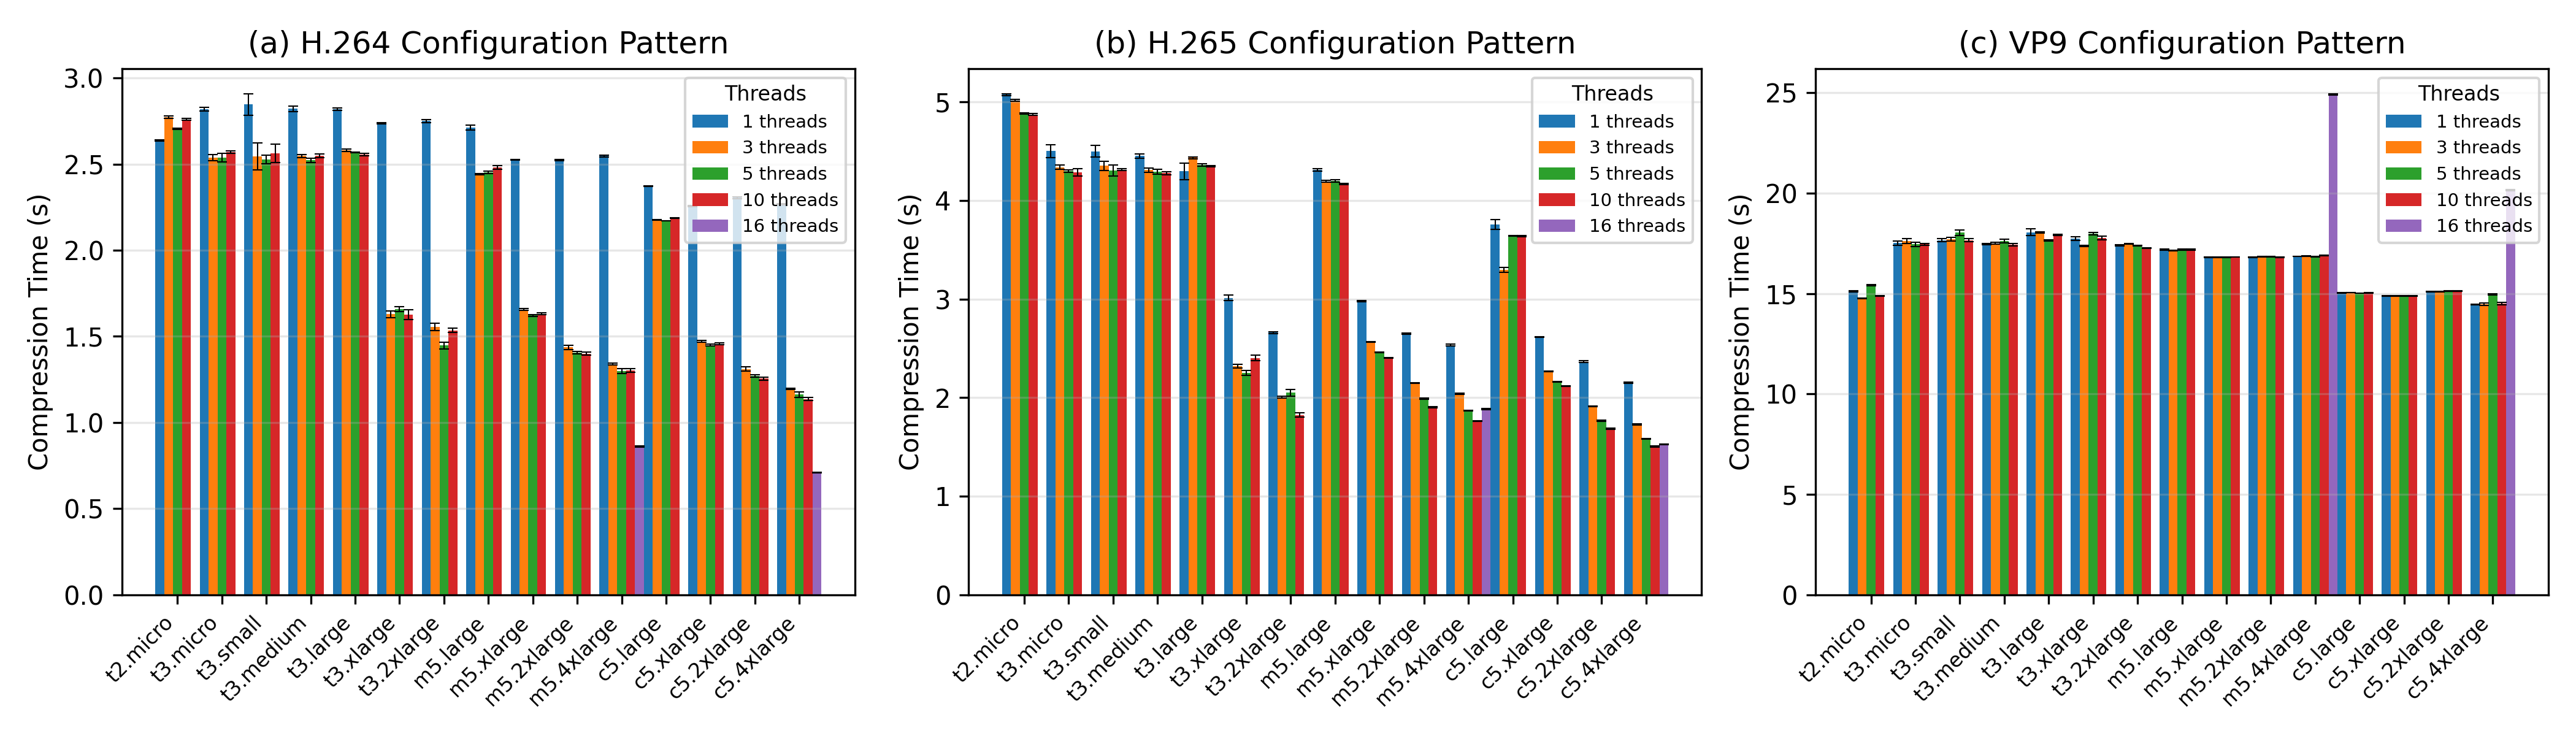
\includegraphics[width=\textwidth]{graphs/unified_codecs_bar_chart.png}
	\caption{Compression time (mean $\pm$ 95\% CI, $n=30$) across all x86 instance
	families for (a) H.264, (b) H.265, and (c) VP9 codecs. Each point represents a distinct instance type within the T, M, or C family. C-family instances
	outperform T and M families at equivalent sizes. Thread scaling yields
	diminishing returns beyond 5 threads for H.264 and H.265 on smaller instances,
	while VP9 exhibits near-constant encoding times up to 10 threads, with
	significant regression at 16 threads on larger configurations.}
	\label{fig:unified_codecs}
\end{figure*}

% -----------------------------------------------------------------------
% PHASE 3 RESULTS
% -----------------------------------------------------------------------
\subsection{Phase 3 Results: Horizontal vs. Vertical Scaling Analysis}

Phase~2 showed \texttt{t3.micro} is the most cost-efficient configuration for H.264 encoding in isolation. Phase~3 tests whether that efficiency holds up at scale---specifically, when a 10-minute video needs to be encoded end-to-end using horizontal (10-node cluster) versus vertical (single large instance) deployment. An important difference in scope: Phase~2 measured raw encoding time on isolated 30-second segments (median $\approx$2.5\,s per segment on \texttt{t3.micro}); Phase~3 measures full pipeline wall-clock time including provisioning, file transfer, encoding, and output retrieval. The higher Phase~3 numbers ($\approx$73\,s per cluster run) do not mean slower encoding---they include $\approx$48\,s of provisioning overhead that Phase~2 never sees.

We use H.264 across all x86 families as the primary scaling benchmark to separate provisioning dynamics from codec-specific noise (Table~\ref{tab:scaling_all_families}). H.265 and VP9 come in for the ARM Graviton comparisons, where codec sensitivity across architectures is the question.

For x86, each 10-node cluster (10$\times$ the smallest instance in a family) goes up against the largest single instance in that family: \texttt{t3.2xlarge}, \texttt{m5.4xlarge}, and \texttt{c5.4xlarge}. The nearest cost-equivalent vertical baseline for the \texttt{t3.micro} cluster (\$0.104/h) would be \texttt{t3.xlarge} (\$0.1664/h), but we deliberately benchmark against the biggest nodes (up to \$0.768/h) to test whether small-instance clusters can outperform---not just match---the highest-throughput option in each tier. ARM Graviton tests were limited to M and C families; we left out T-family Graviton variants (\texttt{t4g}) because their credit mechanics would confound sustained workload comparisons.

\subsubsection{Two-Phase Analysis Results}

Phase~3.1 used stock Ubuntu images with post-boot FFmpeg installation---the simplest possible deployment---to set up an unoptimized baseline for \textbf{RQ2}. The numbers were striking: setup time consumed 57.3--93.3\% of total wall-clock time depending on configuration. Even so, vertical scaling (\texttt{t3.2xlarge}, 3.04 min) edged out the horizontal cluster (\texttt{t3.micro}$\times$10, 3.28 min) by 7.3\%. Where the horizontal cluster won was on cost: \$0.00569 versus \$0.01686 for vertical---a 66.3\% reduction despite being slower. The message was obvious: provisioning overhead is the problem, and fixing it is what Phase~3.2 is for.

Phase~3.2 swapped runtime dependency installation for pre-configured AMIs, targeting \textbf{RQ3}. The improvement was immediate. The optimized \texttt{t3.micro} cluster finished in 1.22 minutes---$1.48\times$ faster than the vertical \texttt{t3.2xlarge} (1.80 min). The same pattern held across larger families: M-family horizontal hit 1.22 min ($1.28\times$ over \texttt{m5.4xlarge} at 1.56 min); C-family hit 1.18 min ($1.26\times$ over \texttt{c5.4xlarge} at 1.49 min). The serial \texttt{t3.micro} baseline was 2.72 min. In every family, the horizontal cluster was both faster and cheaper than the largest vertical instance once provisioning overhead was out of the picture.

\subsubsection{Analysis and Validation}

In parallel configurations, \textit{Effective Encoding Time} covers raw FFmpeg computation plus SFTP segment upload and output retrieval; \textit{Setup Overhead} (used interchangeably with provisioning latency throughout the paper) is the time from the EC2 \texttt{run\_instances} API call until the SSH daemon responds. All experimental artifacts are at \url{https://anonymous.4open.science/r/ec2sweetspot-blinded2}.

Dynamic Phase~3.1 data for 10$\times$\texttt{m5.large} is missing from Table~\ref{tab:scaling_all_families}: all 30 runs hit a systematic FFmpeg muxer overflow on segments~1 and~4, caused by a known bug in the FFmpeg version shipped via Ubuntu~20.04 \texttt{apt}. The bug does not show up in Phase~3.2, which uses a pre-built AMI with a newer FFmpeg build.

Table~\ref{tab:scaling_all_families} has the full timing and cost data for both phases; Figure~\ref{fig:unified_scaling} shows how the gap between horizontal and vertical scaling closes once AMI optimization removes the provisioning bottleneck.

\begin{table*}[!htbp]
\centering
\caption{Scaling strategies across optimization phases. \textbf{Prov.}: Dynamic (Ubuntu) vs.\ Optimized (pre-built AMI). \textbf{Speedup} is relative to the serial baseline of each family and provisioning phase; serial rows are $1.00\times$ by definition. \textbf{Cost$\times$} is total cost relative to the serial AMI baseline. ARM results are in Table~\ref{tab:arm_graviton_scaling}. Dynamic Phase~3.1 data for 10$\times$\texttt{m5.large} is excluded due to systematic FFmpeg muxer overflow (see text).}
\label{tab:scaling_all_families}
\footnotesize
\begin{tabular}{llcccc}
\toprule
\textbf{Instance} & \textbf{Prov.} & \textbf{Time (min)} & \textbf{Cost (USD)} & \textbf{Speedup} & \textbf{Cost$\times$} \\
\midrule
\multicolumn{6}{c}{\textbf{Burstable T} \quad Serial: \texttt{t3.micro} \quad Parallel: 10$\times$\texttt{t3.micro} \quad Vertical: \texttt{t3.2xlarge}} \\
\midrule
\multirow{2}{*}{\texttt{t3.micro}}      & Dynamic   & 4.03 $\pm$ 0.12 & \$0.00070 & 1.00$\times$ & 1.0$\times$ \\
                                         & Optimized & 2.72 $\pm$ 0.08 & \$0.00047 & 1.00$\times$ & 1.0$\times$ \\
\multirow{2}{*}{10$\times$\texttt{t3.micro}} & Dynamic   & 3.28 $\pm$ 0.10 & \$0.00569 & 1.23$\times$ & 8.1$\times$ \\
                                         & Optimized & 1.22 $\pm$ 0.04 & \$0.00211 & 2.23$\times$ & 4.5$\times$ \\
\multirow{2}{*}{\texttt{t3.2xlarge}}    & Dynamic   & 3.04 $\pm$ 0.09 & \$0.01686 & 1.33$\times$ & 24.1$\times$ \\
                                         & Optimized & 1.80 $\pm$ 0.05 & \$0.00998 & 1.51$\times$ & 21.2$\times$ \\
\midrule
\multicolumn{6}{c}{\textbf{General Purpose M} \quad Serial: \texttt{m5.large} \quad Parallel: 10$\times$\texttt{m5.large} \quad Vertical: \texttt{m5.4xlarge}} \\
\midrule
\multirow{2}{*}{\texttt{m5.large}}      & Dynamic   & 3.46 $\pm$ 0.10 & \$0.00554 & 1.00$\times$ & 1.0$\times$ \\
                                         & Optimized & 2.71 $\pm$ 0.08 & \$0.00434 & 1.00$\times$ & 1.0$\times$ \\
10$\times$\texttt{m5.large}               & Optimized & 1.22 $\pm$ 0.04 & \$0.01952 & 2.22$\times$ & 4.5$\times$ \\
\multirow{2}{*}{\texttt{m5.4xlarge}}    & Dynamic   & 2.33 $\pm$ 0.07 & \$0.02982 & 1.48$\times$ & 5.4$\times$ \\
                                         & Optimized & 1.56 $\pm$ 0.05 & \$0.01997 & 1.74$\times$ & 4.6$\times$ \\
\midrule
\multicolumn{6}{c}{\textbf{Compute Optimized C} \quad Serial: \texttt{c5.large} \quad Parallel: 10$\times$\texttt{c5.large} \quad Vertical: \texttt{c5.4xlarge}} \\
\midrule
\multirow{2}{*}{\texttt{c5.large}}      & Dynamic   & 3.21 $\pm$ 0.10 & \$0.00455 & 1.00$\times$ & 1.0$\times$ \\
                                         & Optimized & 2.46 $\pm$ 0.07 & \$0.00349 & 1.00$\times$ & 1.0$\times$ \\
\multirow{2}{*}{10$\times$\texttt{c5.large}} & Dynamic   & 3.52 $\pm$ 0.11 & \$0.04987 & 0.91$\times$ & 11.0$\times$ \\
                                         & Optimized & 1.18 $\pm$ 0.04 & \$0.01672 & 2.08$\times$ & 4.8$\times$ \\
\multirow{2}{*}{\texttt{c5.4xlarge}}    & Dynamic   & 2.13 $\pm$ 0.06 & \$0.02414 & 1.51$\times$ & 5.3$\times$ \\
                                         & Optimized & 1.49 $\pm$ 0.04 & \$0.01689 & 1.65$\times$ & 4.8$\times$ \\
\bottomrule
\end{tabular}
\end{table*}

The Phase~3.2 story is the same across all three families: once provisioning overhead is gone, horizontal clusters are faster \emph{and} cheaper than the largest vertical instance. T-family had the biggest relative speedup: $1.48\times$ (1.22 min vs.\ 1.80 min for \texttt{t3.2xlarge}). M-family: $1.28\times$ (1.22 min vs.\ 1.56 min for \texttt{m5.4xlarge}); C-family: $1.26\times$ (1.18 min vs.\ 1.49 min for \texttt{c5.4xlarge}).

Within-family cost savings are modest in absolute terms: M-family horizontal saved 2.3\% (\$0.01952 vs.\ \$0.01997); C-family saved 1.0\% (\$0.01672 vs.\ \$0.01689). This is expected---per-hour rates for smaller instances within a family scale roughly proportionally to the larger ones, so the main within-family payoff of horizontal scaling is throughput, not cost.

The cost advantage really shows up in cross-family comparisons. Each \texttt{t3.micro} node handles a 60-second chunk in a single burst well within the credit window, delivering 100\% vCPU throughput during encoding---comparable to non-burstable instances for this workload duration. Under these conditions, the \texttt{t3.micro} cluster (\$0.00211) costs 89.4\% less than \texttt{m5.4xlarge} (\$0.01997) and 87.5\% less than \texttt{c5.4xlarge} (\$0.01689), while finishing faster than both.

Worth highlighting: the C-family intra-family result stands on its own. Ten \texttt{c5.large} nodes beat one \texttt{c5.4xlarge} in both speed and cost. Horizontal scaling is not a burstable-instance trick---it is a general property of divisible workloads once provisioning is under control.

Dynamic Phase~3.1 data for 10$\times$\texttt{m5.large} is excluded from Table~\ref{tab:scaling_all_families}: all 30 runs hit a systematic FFmpeg muxer overflow (``too many packets buffered'') on segments~1 and~4, caused by a known bug in the FFmpeg version from Ubuntu~20.04 \texttt{apt}. No complete encoding succeeded. The bug does not appear in Phase~3.2, which uses a pre-built AMI with a patched FFmpeg build---one more reason AMI optimization matters beyond raw provisioning speed.

\begin{figure*}[!ht]
	\centering
	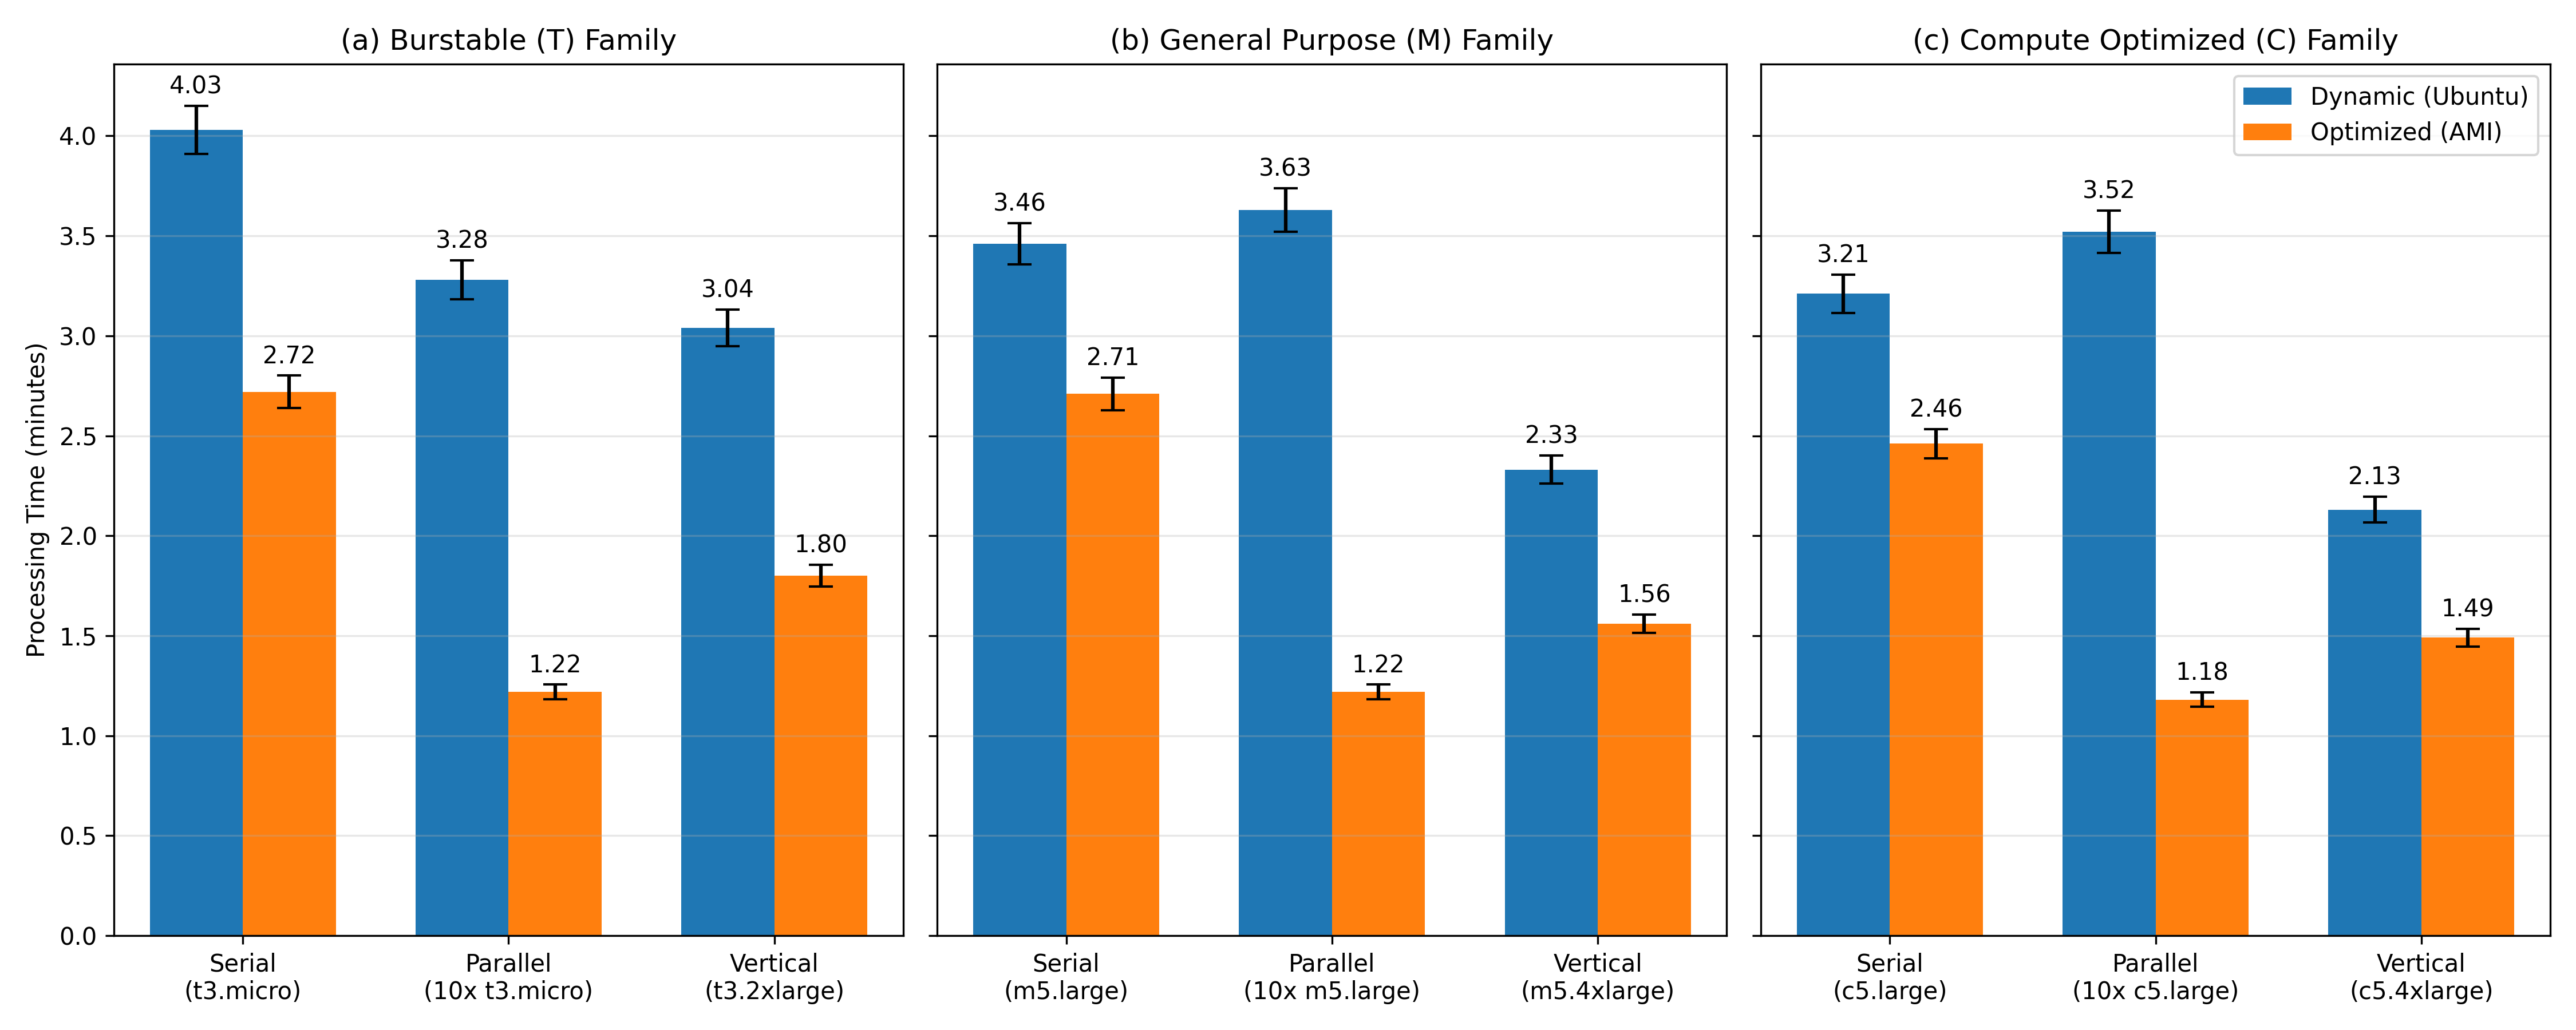
\includegraphics[width=0.7\textwidth]{graphs/unified_scaling_comparison.png}
	\caption{Performance and cost scaling comparison across (a) T, (b) M, and
	(c) C instance families. Left bars: Dynamic provisioning (Phase~3.1); right bars: Optimized AMI (Phase~3.2). Error bars show 95\% CI ($n=30$). The collapse of the performance gap demonstrates horizontal
	scaling speedup when provisioning
	overhead is eliminated.}
	\label{fig:unified_scaling}
\end{figure*}

\subsubsection{Methodological and Statistical Validation}

Welch's t-tests confirm the Phase~3 speedups are real, not variance artifacts: $p < 10^{-23}$ for T-family horizontal vs.\ vertical ($d = 3.74$); $p < 10^{-44}$ for M-family ($d = 8.77$) and C-family ($d = 7.69$). These are large, robust effects. ARM Graviton encoding variance is low once transfer artifacts are factored out: all reconstructed configurations in Table~\ref{tab:arm_graviton_scaling} achieve CV$<$10\%, with provisioning itself measured at CV=1.9\% ($n=100$)---more stable than x86 (CV=4.4\%).

The intra-family comparisons---10$\times$\texttt{m5.large} vs.\ \texttt{m5.4xlarge} and 10$\times$\texttt{c5.large} vs.\ \texttt{c5.4xlarge}---are the cleanest test of the horizontal scaling hypothesis. Both sides are in the same instance family and billing tier, which removes confounds from CPU credit mechanics, cross-family pricing gaps, and heterogeneous workload behavior. The $1.28\times$ and $1.26\times$ speedups in M and C families under these controlled conditions confirm that the advantage is architectural, not an artifact of comparing burstable against non-burstable instances.

The T-family cross-family result (10$\times$\texttt{t3.micro} vs.\ \texttt{m5.4xlarge} or \texttt{c5.4xlarge}) pushes this further: the cost savings (89.4\% and 87.5\%) are large, though part of that gap comes from the pricing difference between burstable and general-purpose families. The intra-family result sets the floor; the cross-family result shows the ceiling for operators willing to mix instance classes.

% -----------------------------------------------------------------------
% EXTENDED EVALUATIONS (M1, M2, M3)
% -----------------------------------------------------------------------
\subsection{Architecture, Codec, and Regional Impact Analysis}

We ran ARM Graviton and regional pricing as independent extensions to the Phase~3 framework, each answering a specific generalizability question: do the x86 findings carry over to a different ISA, and do they hold outside \texttt{us-east-1}?

\textbf{ARM Graviton Performance (Codecs):} Running \texttt{c7g.large} and \texttt{m7g.large} alongside their x86 counterparts turned up interesting architecture-codec interactions. Table~\ref{tab:arm_graviton_scaling} reports reconstructed times (encoding $+$ median provisioning from an independent $n=100$ characterization, factoring out SFTP transfer artifacts). For H.264, \texttt{m7g.large} horizontal scaling gave a $1.72\times$ speedup over serial (33.55\,s vs.\ 57.55\,s), while \texttt{c7g.large} showed no horizontal benefit at all (107.68\,s horizontal $\approx$ 107.41\,s serial). For H.265 the picture flipped: \texttt{c7g.large} horizontal clusters (61.03\,s) crushed \texttt{m7g.large} (182.01\,s)---a $2.98\times$ gap between two ARM instance types. Comparing ARM H.265 against x86 H.264 would be misleading since the codecs differ in computational complexity.

The high H.265 serial times ($\approx$700s for both \texttt{m7g.large} and \texttt{c7g.large}) come down to the computational intensity of \texttt{libx265} \texttt{-preset slow} on ARM: current \texttt{libx265} builds do not have the SIMD optimization depth available on x86, which makes H.265 encoding disproportionately slower on Graviton relative to H.264. For comparison, the same 10-minute H.265 encoding on x86 (\texttt{c5.large} serial) finishes in $\approx$72s---an order of magnitude faster---underscoring the architecture--codec interaction.

Table~\ref{tab:arm_graviton_scaling} has Phase~3.2 results for all ARM configurations. Two H.265 serial rows have an adjusted $n$: isolated container orchestration anomalies caused complete pipeline stalls in a handful of \texttt{m7g.large} and \texttt{c7g.large} runs, producing extreme outliers ($>$5 standard deviations from the mean). We excluded those corrupted runs to keep the central tendency analysis meaningful, yielding $n=26$ (\texttt{m7g.large}) and $n=29$ (\texttt{c7g.large}). The resulting \texttt{m7g.large} H.265 serial distribution is unimodal with low variance (median 700.51s, stdev 4.10s).

\begin{table*}[h]
	\centering
	\caption{Descriptive statistics for compression time (seconds), efficiency, and total cost for ARM Graviton configurations. Horizontal and serial H.264/VP9 times are reconstructed from measured encoding time plus the median provisioning latency from an independent $n=100$ characterization experiment (20.5\,s, CV=1.9\%), isolating cloud-side variance from local transfer artifacts.$^{\dagger}$H.265 serial statistics adjusted after excluding extreme outliers caused by isolated container orchestration failures ($n=26$ for m7g.large; $n=29$ for c7g.large). All rows use $n=30$ encoding measurements.}
	\label{tab:arm_graviton_scaling}
	\resizebox{\textwidth}{!}{%
		\begin{tabular}{ll|rrrr|rrrr|rrrr}
			\toprule
			& & \multicolumn{4}{c|}{H.264} & \multicolumn{4}{c|}{H.265 (libx265)} & \multicolumn{4}{c}{VP9 (libvpx-vp9)} \\
			\cmidrule(lr){3-6} \cmidrule(lr){7-10} \cmidrule(lr){11-14}
			& & \multicolumn{3}{c}{Compression Time (s)} & \multicolumn{1}{c|}{Eff. | Cost (\$)} & \multicolumn{3}{c}{Time (s)} & \multicolumn{1}{c|}{Eff. | Cost (\$)} & \multicolumn{3}{c}{Time (s)} & \multicolumn{1}{c}{Eff. | Cost (\$)} \\
			Instance Type & Strategy & Median & Std & CV(\%) & (Median) & Median & Std & CV(\%) & (Median) & Median & Std & CV(\%) & (Median) \\
			\midrule
			m7g.large & serial & \textbf{57.5500} & 0.61 & 1.1 & \textbf{13} | \textbf{0.0013045} & 700.5100$^{\dagger}$ & 4.10 & 0.6 & 0 | 0.0158782 & 329.0300 & 1.41 & 0.4 & 0 | 0.0074580 \\
			m7g.large & horizontal & 33.5500 & 3.04 & 8.8 & \textbf{131} | \textbf{0.0076047} & \textbf{182.0050} & 11.39 & 6.2 & \textbf{242} | \textbf{0.0041254} & 63.0961 & 2.53 & 4.0 & 69 | 0.0143018 \\
			\cmidrule(lr){1-14}
			c7g.large & serial & \textbf{107.4101} & 1.79 & 1.7 & \textbf{462} | \textbf{0.0021631} & 702.1500$^{\dagger}$ & 1.36 & 0.2 & 0 | 0.0141405 & 328.7450 & 1.60 & 0.5 & 0 | 0.0066114 \\
			c7g.large & horizontal & 107.6800 & 18.34 & 17.0 & 4 | 0.0021656 & \textbf{61.0300} & 2.76 & 4.5 & \textbf{13} | \textbf{0.0012274} & \textbf{63.2736} & 6.02 & 9.3 & \textbf{78} | \textbf{0.0127426} \\
			\bottomrule
		\end{tabular}%
	}
\end{table*}

\textbf{Statistical Validation:} Welch's t-test found no significant difference between \texttt{m7g.large} and \texttt{c7g.large} for H.265 horizontal encoding ($p > .05$), with moderate variability (CV 4.5--6.2\%) in H.265 horizontal runs. A Mann-Whitney U test agreed ($p > .05$), providing non-parametric confirmation. Welch's t-test did confirm the H.264 inversion on \texttt{m7g.large} at high confidence ($p < 10^{-12}$, Cohen's $d = 4.31$): this is not noise but a structural effect of provisioning overhead dominating encoding time at this chunk granularity.

To separate cloud-side variance from local experimental artifacts (SFTP transfer contention), Table~\ref{tab:arm_graviton_scaling} reports reconstructed times: measured encoding duration plus the median provisioning latency from an independent $n=100$ experiment (20.5\,s, CV=1.9\% for ARM Graviton---more stable than x86 at CV=4.4\%). Under this decomposition, all ARM configurations have CV$<$10\%.

\textbf{Regional Cost Disparities:} Running the same experiments in \texttt{sa-east-1} (S\~{a}o Paulo) revealed a 54--62\% price premium over \texttt{us-east-1}, varying by family (T: +61.5\%, M: +59.4\%, C: +54.1\%). For H.264 horizontal deployments (10$\times$ nodes, 60s chunks), cluster costs roughly double: \texttt{t3.micro} \$0.0021 vs.\ \$0.0045; \texttt{m5.large} \$0.0150 vs.\ \$0.0339; \texttt{c5.large} \$0.0152 vs.\ \$0.0234. Wall-clock times stayed the same across regions, confirming that compute performance is hardware-bound, not region-bound---the cost difference is purely a pricing artifact.

\subsection{Phase 4 Results: Chunk Size Sensitivity and Cost Analysis}
\label{results-phase4}

Phase~4 adds two analyses that address \textbf{RQ4}: an empirical study of chunk duration sensitivity and a cost model for network egress.

\textbf{Chunk Size Sensitivity:}
Total wall-clock time for a horizontally scaled cluster depends on chunk duration $c$ in a non-monotone way. For a video of length $L$ processed across $N = \lceil L/c \rceil$ parallel instances:
\begin{equation}
T(c) = t_{\text{seg}} + \max_{1 \le i \le N} \left( t_{\text{prov},i} \right) + t_{\text{enc}}(c) + t_{\text{merge}}
\end{equation}
Shorter chunks mean more instances ($N$ goes up), which widens the expected maximum provisioning time---the synchronization barrier at the end of the parallel phase. Longer chunks mean fewer workers and less parallelism, making encoding time the bottleneck. We measured this trade-off at $c \in \{30, 60, 120\}$s on the 10-minute H.264 workload with the Phase~3.2 AMI across all three x86 families. Total Time in Table~\ref{tab:chunk_sensitivity} is end-to-end wall-clock; speedup is relative to each family's vertical baseline (\texttt{t3.2xlarge}: 1.80\,min; \texttt{m5.4xlarge}: 1.56\,min; \texttt{c5.4xlarge}: 1.49\,min).

For 240p content, 60-second chunks were optimal across the board: 30-second chunks hurt performance because 20 provisioning sequences widen the long-tail outlier; 120-second chunks left only 5 workers, not enough parallelism. At 60s, speedup over the vertical baseline reached 1.48$\times$ (T), 1.28$\times$ (M), and 1.26$\times$ (C).

\textbf{Resolution Dependence:} To check whether this optimum holds beyond low-resolution workloads, we replicated the M-family chunk sensitivity experiment at 720p and 1080p using \texttt{m5.large} horizontal clusters (Table~\ref{tab:chunk_multiresolution}). Turns out the optimal chunk size shifts with resolution: at 240p, where per-chunk encoding ($\approx$5\,s) is dwarfed by provisioning ($\approx$18\,s), 60-second chunks hit the right balance between parallelism and provisioning overhead. At 720p and 1080p, encoding time grows by $10\times$ and $30\times$ respectively, so parallelism matters more---30-second chunks become optimal because the extra provisioning cost is amortized over much longer per-chunk encoding. SFTP transfer overhead also scales with chunk file size, adding 26--199\,s per chunk at higher resolutions; an S3-based pipeline would shrink this but was not tested.

\begin{table}[h]
	\centering
	\caption{Chunk size sensitivity across resolutions (M-family, \texttt{m5.large} horizontal, H.264, single trial). Boldface marks the fastest configuration per resolution.}
	\label{tab:chunk_multiresolution}
	\resizebox{\columnwidth}{!}{
		\begin{tabular}{|l|c|c|c|c|}
			\hline
			\textbf{Resolution} & \textbf{Chunk} & \textbf{Total (min)} & \textbf{Avg Encode (s)} & \textbf{Avg Upload (s)} \\
			\hline
			\multirow{3}{*}{240p (320$\times$240)} & \textbf{30s} & 1.63 & $\approx$5 & $<$1 \\
			& \textbf{60s} & \textbf{1.22} & $\approx$5 & $<$1 \\
			& 120s & 2.10 & $\approx$5 & $<$1 \\
			\hline
			\multirow{3}{*}{720p (1280$\times$720)} & \textbf{30s} & \textbf{4.12} & 50.6 & 66.2 \\
			& 60s & 5.31 & 95.5 & 128.6 \\
			& 120s & 7.73 & 199.9 & 135.1 \\
			\hline
			\multirow{3}{*}{1080p (1920$\times$1080)} & \textbf{30s} & \textbf{5.49} & 129.8 & 21.9 \\
			& 60s & 6.40 & 219.7 & 48.6 \\
			& 120s & 9.00 & 371.7 & 52.0 \\
			\hline
		\end{tabular}
	}
\end{table}

\begin{table}[h]
	\centering
	\caption{Chunk size sensitivity: wall-clock time and speedup over vertical baseline.}
	\label{tab:chunk_sensitivity}
	\resizebox{\columnwidth}{!}{
		\begin{tabular}{|l|l|c|c|}
			\hline
			\textbf{Family} & \textbf{Chunk Strategy} & \textbf{Total Time (min)} & \textbf{Speedup vs Vertical} \\
			\hline
			\multirow{3}{*}{Burstable (T)} & 30s (20x t3.micro) & 1.39 & 1.30$\times$ \\
			& \textbf{60s (10x t3.micro)} & \textbf{1.22} & \textbf{1.48$\times$} \\
			& 120s (5x t3.micro) & 2.04 & 0.88$\times$$^{*}$ \\
			\hline
			\multirow{3}{*}{General (M)} & 30s (20x m5.large) & 1.63 & 0.96$\times$$^{*}$ \\
			& \textbf{60s (10x m5.large)} & \textbf{1.22} & \textbf{1.28$\times$} \\
			& 120s (5x m5.large) & 2.10 & 0.74$\times$$^{*}$ \\
			\hline
			\multirow{3}{*}{Compute (C)} & 30s (20x c5.large) & 1.44 & 1.03$\times$ \\
			& \textbf{60s (10x c5.large)} & \textbf{1.18} & \textbf{1.26$\times$} \\
			& 120s (5x c5.large) & 1.98 & 0.75$\times$$^{*}$ \\
			\hline
			\multicolumn{4}{|l|}{\footnotesize $^{*}$ Speedup $< 1.0\times$ indicates horizontal cluster is \textit{slower} than vertical.} \\
			\hline
		\end{tabular}
	}
\end{table}

\textbf{The Network Egress Economic Bottleneck:}
Optimized chunking brings compute costs down, but a full cloud pipeline cost picture needs a deterministic model. Total Cost ($C_{\text{total}}$) is the sum of compute provisioning ($C_{\text{comp}}$) and outbound data transfer ($C_{\text{net}}$) (Eq.~\ref{eq:cost_model}):
\begin{equation}
\label{eq:cost_model}
C_{\text{total}} = \left( \sum_{i=1}^{N} R_{\text{inst}} \times T_{i} \right) + \left( R_{\text{egress}} \times D_{\text{out}} \right)
\end{equation}
where $R_{\text{inst}}$ is the per-second instance billing rate, $T_i$ is the active billing lifespan of node $i$,\footnote{AWS imposes a 60-second minimum billing floor per instance: any $T_i < 60$\,s is billed as 60\,s. All $T_i$ values observed in our experiments exceed this threshold.} $R_{\text{egress}}$ is the regional outbound internet data transfer rate (e.g., \$0.09/GB in \texttt{us-east-1}, \$0.25/GB in \texttt{sa-east-1}), and $D_{\text{out}}$ is the final payload size in GB.

Intra-region transfers carry no additional per-GB charges. Outbound internet egress, on the other hand, sets a hard economic floor: delivering the $\approx$100\,MB H.264 output costs $\approx$\$0.009 in \texttt{us-east-1} ($\approx$4$\times$ the optimized \texttt{t3.micro} compute cost of \$0.00211), which makes egress the dominant cost once compute is optimized.

Routing delivery through a CDN (S3\,+\,CloudFront) cuts this by $\approx$10$\times$: CloudFront charges \$0.0085/GB vs.\ \$0.09/GB for direct egress, making CDN delivery cheaper than compute above $\approx$2\,GB/month of output.

% -----------------------------------------------------------------------
% DISCUSSION AND THREATS TO VALIDITY
% -----------------------------------------------------------------------
\section{Discussion and Threats to Validity}
\label{limitations}

The results back optimized horizontal scaling as a practical cost reduction strategy. Below we discuss the main constraints and threats to generalizability.

\textbf{AMI vs.\ runtime-install overhead:} In Phase~3.2, FFmpeg and all dependencies are baked into the custom AMI; nothing gets installed at runtime. The remaining provisioning overhead ($\approx$48\,s) is just EC2 launch, EBS volume attachment, OS boot, and SSH readiness. In Phase~3.1, FFmpeg is installed post-boot via \texttt{apt}, which explains the much higher setup times. These two phases are not interchangeable baselines.

\textbf{Burstable CPU credit surcharges:} T-family instances run in Unlimited mode~\cite{awscredits} and start drawing Surplus Credits the moment they launch. Since our orchestration pattern is strictly ephemeral (spawn, encode, terminate), instances never sit idle long enough to offset that draw. Rather than reporting a single surcharge figure, we bound it: under a realistic encoding-focused assumption ($\approx$22\,s at full CPU), the per-cluster surcharge is $\approx$\$0.0055, bringing cluster cost to $\approx$\$0.0076---still 62\% below \texttt{m5.4xlarge}. In the worst case (100\% CPU for the full 73\,s wall time), the surcharge hits $\approx$\$0.0183 and wipes out the cost advantage entirely. We did not audit billing statements; the true value falls somewhere between these bounds depending on actual CPU utilization during non-encoding phases.

\textbf{Alternative baselines:} We tested on-demand EC2 with custom orchestration. AWS-native services (Elemental MediaConvert, Fargate) get near-zero provisioning overhead by design; spot instances~\cite{b21,b19} are cheaper but come with preemption risk. Both comparisons are left for future work.

\textbf{Transfer overhead:} We used SFTP for chunk distribution within a single AZ. Horizontal configurations transfer $N$ chunks simultaneously from the orchestrating host, while vertical transfers just one file, so SFTP penalizes horizontal scaling relative to what an S3-based pipeline would achieve. The speedup advantages we report are therefore conservative lower bounds.

\textbf{Scope:} Multi-resolution replication (720p, 1080p) confirmed resolution-dependent chunk optima (Table~\ref{tab:chunk_multiresolution}). ARM homogeneity was validated in \texttt{us-east-1} only. All shared-tenancy instances are subject to noisy-neighbor effects (mitigated by CV$<$0.6\% and $n=30$). Pricing and hardware generations change; absolute figures should be re-validated before production use.

% -----------------------------------------------------------------------
% CONCLUSION
% -----------------------------------------------------------------------
\section{Conclusion}
\label{conclusion}

For short-form video encoding on EC2, the biggest cost driver is not the CPU---it is waiting for instances to become ready. Provisioning overhead consumed up to 93.3\% of wall-clock time in unoptimized horizontal deployments, wiping out burstable-instance cost advantages entirely. Getting rid of that overhead via workload-optimized AMIs let a 10-node \texttt{t3.micro} cluster beat a single \texttt{m5.4xlarge} by $1.28\times$ at 89.4\% lower base-compute cost---and the result held within families as well. ARM Graviton clusters reached competitive H.265 horizontal performance (median 61.03\,s on \texttt{c7g.large}, CV=4.5\%). Multi-resolution tests showed the optimal chunk size depends on resolution: 60\,s for 240p but 30\,s for 720p and 1080p, where encoding time outweighs provisioning. Once compute is optimized, outbound egress becomes the binding cost constraint. Fixing provisioning overhead is the prerequisite for cost-effective horizontal cloud transcoding; GPU-accelerated instances and spot pricing are the most promising next steps.

% APPENDIX removed — submitted as separate document
% -----------------------------------------------------------------------
%\appendices
%\section{Artifact Documentation: EC2 Sweet Spot}
%\label{app:artifact}

%This appendix documents the research artifacts for the ``EC2 Sweet Spot'' study
%on Amazon EC2 instance selection for video compression workloads. All
%experimental materials are available at
%\url{https://anonymous.4open.science/r/ec2sweetspot-blinded2}.
%
%\subsection{Artifact Overview}
%
%The artifact collection contains:
%\begin{itemize}
%	\item Complete experimental setup and configuration files
%	\item Raw and processed performance data from over 4,100 instance deployments
%	\item Benchmarking scripts for performance evaluation
%	\item Data processing pipelines for statistical analysis
%	\item Reproduction scripts for all experimental phases
%\end{itemize}
%
%\subsection{Experimental Methodology}
%
%The artifact supports four experimental phases:
%
%\textbf{Phase 1: Hardware Homogeneity Validation}
%\begin{itemize}
%	\item CPU model verification across 6 AWS availability zones
%	\item Analysis of processor distribution patterns
%	\item Automatic retry mechanisms for hardware validation
%\end{itemize}
%
%\textbf{Phase 2: Performance Benchmarking}
%\begin{itemize}
%	\item Evaluation of 15 EC2 instance types (7 T-family including t2.micro, 4 M-family, 4 C-family)
%	\item Three video codecs (H.264, H.265, VP9) with 4 thread configurations
%	\item 30 iterations per configuration for statistical significance
%	\item Cost-efficiency calculations based on AWS pricing
%\end{itemize}
%
%\textbf{Phase 3: Scaling Strategy Analysis}
%\begin{itemize}
%	\item Comparison of horizontal vs.\ vertical scaling approaches
%	\item Dynamic provisioning vs.\ optimized AMI deployment
%	\item Complete workflow timing and cost analysis
%\end{itemize}
%
%\subsection{Data Collection}
%
%The artifact includes:
%\begin{itemize}
%	\item Over 4,100 CPU verification logs from \texttt{/proc/cpuinfo}
%	\item Over 60 structured execution logs with detailed timing information
%	\item 9 CSV files with aggregated performance metrics
%	\item Raw timing data for over 6,500 benchmark executions (Phase~2: $15 \times 4 \times 3 \times 30 = 5{,}400$; Phase~3 x86 scaling: $\approx$540; ARM Graviton: $\approx$240; Phase~4 chunk sensitivity: $\approx$270; sa-east-1 regional: 90)
%\end{itemize}
%
%\subsection{Reproduction Requirements}
%
%\textbf{Infrastructure:}
%\begin{itemize}
%	\item AWS EC2 access in \texttt{us-east-1} and \texttt{sa-east-1} regions
%	\item Support for 17 EC2 instance types: 15 x86 (7 T-family including t2.micro, 4 M-family, 4 C-family) and 2 ARM Graviton 3 (m7g.large, c7g.large)
%	\item Ubuntu 22.04 LTS base AMI (\texttt{us-east-1}: ami-0a313d6098716f372; AMI IDs are region-specific---for \texttt{sa-east-1} and ARM configurations, use the equivalent Ubuntu 22.04 LTS AMI for that region, available via AWS EC2 AMI catalog)
%	\item Custom AMI with pre-installed dependencies (\texttt{us-east-1}: ami-0300cfb109571fb0b; equivalent AMIs must be built for other regions using the provided Packer/setup scripts in the artifact repository)
%\end{itemize}
%
%\textbf{Software Dependencies:}
%\begin{itemize}
%	\item Python 3.8+ with boto3, paramiko, pandas, numpy, matplotlib
%	\item Docker for containerized FFmpeg execution
%	\item AWS CLI with appropriate EC2 permissions
%\end{itemize}
%
%\textbf{Estimated Reproduction Cost:} \$400--\$600 (AWS instance hours, breakdown: Phase~2 benchmarks $\approx$\$50--\$80; Phase~3 x86 scaling $\approx$\$100--\$150; ARM Graviton evaluation $\approx$\$80--\$120; sa-east-1 regional replication $\approx$\$60--\$100; Phase~4 chunk sensitivity $\approx$\$40--\$60; data transfer and miscellaneous $\approx$\$30--\$60). Note: costs scale with AWS pricing at time of reproduction and may vary by region.\\
%\textbf{Estimated Time:} 4--6 days for complete reproduction
%
%\subsection{Artifact Structure}
%
%The repository contains the following components:
%\begin{itemize}
%	\item \texttt{experimental\_data/} --- Processed results in CSV format
%	\item \texttt{phase1\_homogeneity/} --- CPU validation data and analysis
%	\item \texttt{phase2\_benchmarks/} --- Performance benchmarking scripts
%	\item \texttt{phase3\_scaling/} --- Scaling strategy analysis scripts
%	\item \texttt{scripts/processing/} --- Data analysis pipelines
%	\item \texttt{test\_videos/} --- Benchmark media files (20\,MB, 51\,MB, 2.5\,MB)
%	\item \texttt{documentation/} --- Reproduction guides and validation
%\end{itemize}
%
%\subsection{Extended Evaluations}
%
%The artifact repository also documents two extended experiments conducted beyond the core x86 Phase~3 scaling analysis:
%
%\textbf{ARM Graviton Extended Evaluation:} Scripts and raw data for the \texttt{m7g.large} and \texttt{c7g.large} experiments (H.264, H.265, and VP9 codecs, serial and horizontal strategies) are located in \texttt{phase3\_scaling/arm\_graviton/}. The ARM AMI configuration and CPU verification scripts are documented in \texttt{phase3\_scaling/arm\_setup.md}. Note that ARM AMI IDs differ from x86 IDs and must be resolved separately for each target region.
%
%\textbf{Regional Pricing Evaluation (\texttt{sa-east-1}):} Scripts and processed results for the São Paulo region replication (H.264 horizontal, \texttt{t3.micro}, \texttt{m5.large}, \texttt{c5.large}) are in \texttt{phase3\_scaling/sa\_east\_1/}. The 44\% regional price premium is captured in the experimental configuration files under \texttt{experimental\_data/regional/}.
%
%\subsection{Validation}
%
%All experimental results in the main paper can be reproduced using the artifact
%repository at \url{https://anonymous.4open.science/r/ec2sweetspot-blinded2}, the
%reproduction scripts in \texttt{scripts/processing/}, and the validation
%procedures documented in \texttt{CHECKLIST.md}. The artifact provides complete
%methodological transparency and enables independent verification of all findings
%presented in this work.
%
% -----------------------------------------------------------------------
% BIBLIOGRAPHY
% -----------------------------------------------------------------------
\begin{thebibliography}{00}

\bibitem{b1} W. Maas, F. Rossi, M. Caggiani, P. Navaux, and A. Lorenzon,
``Investigating cloud instances to achieve optimal trade-offs between
performance-cost efficiency,'' \emph{Computing}, vol. 107, no. 1,
pp. 82--97, Jan. 2025. doi: 10.1007/s00607-025-01444-9.

\bibitem{b2} P. Álvarez, S. Hernández, J. Fabra, and J. Ezpeleta,
``Cost-driven provisioning and execution of a computing-intensive service on
the Amazon EC2,'' \emph{The Computer Journal}, vol. 61, no. 9,
pp. 1407--1421, Jan. 2018. doi: 10.1093/comjnl/bxy006.

\bibitem{b3} T. Dancheva, U. Alonso, and M. D. Barton, ``Cloud benchmarking
and performance analysis of an HPC application in Amazon EC2,''
\emph{Cluster Computing}, vol. 27, no. 2, pp. 2273--2290, Jun. 2023.
doi: 10.1007/s10586-023-04060-4.

\bibitem{b4} L. M. Haji, S. R. M. Zeebaree, O. M. Ahmed, A. B. Sallow,
K. Jacksi, and R. R. Zeabri, ``Dynamic Resource Allocation for Distributed
Systems and Cloud Computing,'' \emph{Test Engineering and Management},
vol. 83, no. 1, pp. 22417--22426, Jun. 2020.

\bibitem{b5} Z. Ou, H. Zhuang, J. K. Nurminen, A. Ylä-Jääski, and P. Hui,
``Exploiting Hardware Heterogeneity within the Same Instance Type of Amazon
EC2,'' in \emph{Proc. 4th USENIX Conf. Hot Topics Cloud Comput.}, Boston,
MA, USA, 2012, pp. 4--4.

\bibitem{b6} Z. Ou, H. Zhuang, A. Lukyanenko, J. K. Nurminen, P. Hui,
V. V. Mazalov, and A. Ylä-Jääski, ``Is the Same Instance Type Created Equal?
Exploiting Heterogeneity of Public Clouds,'' \emph{IEEE Trans. Cloud Comput.},
vol. 1, no. 2, pp. 201--214, Jan. 2013. doi: 10.1109/TCC.2013.12.

\bibitem{b7} B. Farley, A. Juels, V. Varadarajan, T. Ristenpart, K. D. Bowers,
and M. M. Swift, ``More for Your Money: Exploiting Performance Heterogeneity
in Public Clouds,'' in \emph{Proc. 3rd ACM Symp. Cloud Comput.}, San Jose,
CA, USA, 2012, pp. 20:1--20:14. doi: 10.1145/2391229.2391249.

\bibitem{b8} A. Katsenou, X. Wang, D. Schien, and D. Bull, ``Comparative Study
of Hardware and Software Power Measurements in Video Compression,'' in
\emph{2024 Picture Coding Symp. (PCS)}, Taichung, Taiwan, 2024, pp. 1--5.
doi: 10.1109/PCS60826.2024.10566286.

\bibitem{b9} A. Pereira Ferreira and R. O. Sinnott, ``A Performance Evaluation
of Containers Running on Managed Kubernetes Services,'' in \emph{2019 IEEE
Int. Conf. Cloud Comput. Technol. Sci. (CloudCom)}, Sydney, Australia, 2019,
pp. 199--208. doi: 10.1109/CloudCom.2019.00038.

\bibitem{b10} J. Scheuner and P. Leitner, ``Estimating Cloud Application
Performance Based on Micro-Benchmark Profiling,'' in \emph{2018 IEEE 11th
Int. Conf. Cloud Comput. (CLOUD)}, San Francisco, CA, USA, 2018, pp. 90--97.
doi: 10.1109/CLOUD.2018.00019.

\bibitem{b11} S. Ebneyousef and S. Ghazanfari-Rad, ``Cloud Resource Demand
Prediction to Achieve Efficient Resource Provisioning,'' in \emph{2022 8th
Iranian Conf. Signal Process. Intell. Syst. (ICSPIS)}, Tehran, Iran, 2022,
pp. 1--6. doi: 10.1109/ICSPIS56952.2022.10043900.

\bibitem{b12} T. S. Nikoui, A. Balador, A. M. Rahmani, and Z. Bakhshi,
``Cost-Aware Task Scheduling in Fog-Cloud Environment,'' in \emph{2020
CSI/CPSSI Int. Symp. Real-Time Embedded Syst. Technol. (RTEST)}, Tehran,
Iran, 2020, pp. 1--8. doi: 10.1109/RTEST49666.2020.9140118.

\bibitem{b13} Y. Yang and H. Casanova, ``RUMR: Robust Scheduling for Divisible
Workloads,'' in \emph{Proc. 12th IEEE Int. Symp. High Perform. Distrib.
Comput.}, Seattle, WA, USA, 2003, pp. 114--123.
doi: 10.1109/HPDC.2003.1210021.

\bibitem{b14} J. Praveenchandar and A. Tamilarasi, ``Resource Allocation Using
Phase Change Hyper Switching Algorithm in the Cloud Environment,''
\emph{Intell. Autom. Soft Comput.}, vol. 34, no. 3, pp. 1839--1850,
Aug. 2022. doi: 10.32604/iasc.2022.026354.

\bibitem{b15} R. Rosado, O. Santos, F. Oliveira, L. Silva, G. Sanchez,
I. Storch, D. Palomino, and L. Agostini, ``A Coding-Efficiency-Aware Fast
Heuristic for VVC Intra-Frame Prediction Targeting 360° Videos,'' in
\emph{Proc. 30th Brazilian Symp. Multimedia Web}, Juiz de Fora, Brazil, 2024,
pp. 355--359. doi: 10.5753/webmedia.2024.243128.

\bibitem{b16} L. Araújo, A. Duarte, G. Correa, B. Zatt, and D. Palomino,
``Fast ISP Mode Decision for the Versatile Video Coding Intra Prediction Using
Machine Learning,'' in \emph{Proc. 30th Brazilian Symp. Multimedia Web},
Juiz de Fora, Brazil, 2024, pp. 162--170. doi: 10.5753/webmedia.2024.243129.

\bibitem{b17} A. Mahida, ``Comprehensive Review on Optimizing Resource
Allocation in Cloud Computing for Cost Efficiency,'' \emph{J. Artif. Intell.
Cloud Comput.}, vol. 1, no. 2, pp. 1--4, May 2022.
doi: 10.47363/JAICC/2022(1)232.

\bibitem{b18} O. Alzakholi, L. M. Haji, H. M. Shukur, R. R. Zebari,
S. M. Abas, and M. Sadeeq, ``Comparison Among Cloud Technologies and Cloud
Performance,'' \emph{J. Appl. Sci. Technol. Trends}, vol. 1, no. 1,
pp. 40--47, Apr. 2020. doi: \url{https://doi.org/10.38094/jastt1219}.

\bibitem{b19} O. A. Ben-Yehuda, M. Ben-Yehuda, A. Schuster, and D. Tsafrir,
``Deconstructing Amazon EC2 Spot Instance Pricing,''
\emph{ACM Trans. Econ. Comput.}, vol.\ 1, no.\ 3, pp.\ 16:1--16:20, Sep.\ 2013.
doi: 10.1145/2509413.2509416.

\bibitem{b20} F. Jiang, K. Ferriter, and C. Castillo, ``A Cloud-Agnostic
Framework to Enable Cost-Aware Scheduling of Applications in a Multi-Cloud
Environment,'' in \emph{2020 IEEE/IFIP Network Operations and Management
Symposium (NOMS)}, Budapest, Hungary, 2020, pp. 1--9.
doi: 10.1109/NOMS47738.2020.9110325.

\bibitem{b21} A. Zabrovskiy, P. Agrawal, V. Kashansky, R. Kersche,
C. Timmerer, and R. Prodan, ``FSpot: Fast and Efficient Video Encoding
Workloads Over Amazon Spot Instances,'' \emph{Computers, Materials \&
Continua}, vol. 71, no. 3, pp. 5677--5694, 2022.
doi: 10.32604/cmc.2022.023630.

\bibitem{b22} W. Moina-Rivera, M. Garcia-Pineda, J. Gutiérrez-Aguado, and
J. M. Alcaraz-Calero, ``Cloud media video encoding: review and challenges,''
\emph{Multimedia Tools and Applications}, vol. 83, pp. 81231--81278, 2024.
doi: 10.1007/s11042-024-18763-2.

\bibitem{b23} W. Maas, F. D. Rossi, M. C. Luizelli, P. O. A. Navaux, and
A. F. Lorenzon, ``Towards Optimizing Cost and Performance for Parallel
Workloads in Cloud Computing,'' in \emph{Proc. 15th Int. Conf. Cloud Comput.
and Services Science (CLOSER)}, 2025, pp. 231--238.
doi: \url{https://doi.org/10.5220/0013421600003950}.


\bibitem{awscredits} Amazon Web Services, ``Burstable performance instances,''
\emph{Amazon EC2 User Guide}, 2024. [Online]. Available:
\url{https://docs.aws.amazon.com/AWSEC2/latest/UserGuide/burstable-performance-instances.html}
[Accessed: Mar.\ 2026].

\bibitem{dockercoldstart} W. Felter, A. Ferreira, R. Rajamony, and J. Rubio,
``An Updated Performance Comparison of Virtual Machines and Linux Containers,''
in \emph{2015 IEEE Int. Symp. Perform. Anal. Syst. Softw. (ISPASS)},
Philadelphia, PA, USA, 2015, pp. 171--172.
doi: 10.1109/ISPASS.2015.7095802.

\bibitem{awsgrav3} Amazon Web Services, ``AWS Graviton3 Processor,''
\emph{Amazon EC2 Product Page}, 2022. [Online]. Available:
\url{https://aws.amazon.com/ec2/graviton/}
[Accessed: Mar.\ 2026].

\bibitem{neonvideo} MulticoreWare Inc., ``x265 HEVC Encoder Documentation: Architecture-specific Optimizations,''
\emph{x265 Project Documentation}, 2023. [Online]. Available:
\url{https://x265.readthedocs.io/en/master/}
[Accessed: Mar.\ 2026].

\bibitem{excamera} S. Fouladi, R. S. Wahby, B. Shacklett, K. V. Balasubramaniam,
W. Zeng, R. Bhalerao, A. Sivaraman, G. Porter, and K. Winstein,
``Encoding, Fast and Slow: Low-Latency Video Processing Using Thousands
of Tiny Threads,'' in \emph{Proc. 14th USENIX Symp. Networked Systems
Design and Implementation (NSDI)}, Boston, MA, Mar.\ 2017, pp.\ 363--376.
[Online]. Available: \url{https://www.usenix.org/conference/nsdi17/technical-sessions/presentation/fouladi}
[Accessed: Mar.\ 2026].

\bibitem{awsmediaconvert} Amazon Web Services, ``AWS Elemental MediaConvert,''
\emph{AWS Documentation}, 2024. [Online]. Available:
\url{https://aws.amazon.com/mediaconvert/}
[Accessed: Mar.\ 2026].

\end{thebibliography}

\end{document}